\chapter{Pattern Formation}
Examples of the importance of spatial patterning and structure can be seen just about everywhere in the natural world \see{Pattern_examples}. Here, we will be concerned with building and analysing models which can generate such patterns. Specifically, we want to see how simplicity can lead to complexity.
\begin{figure}[!!!h!!!tb]
\centering
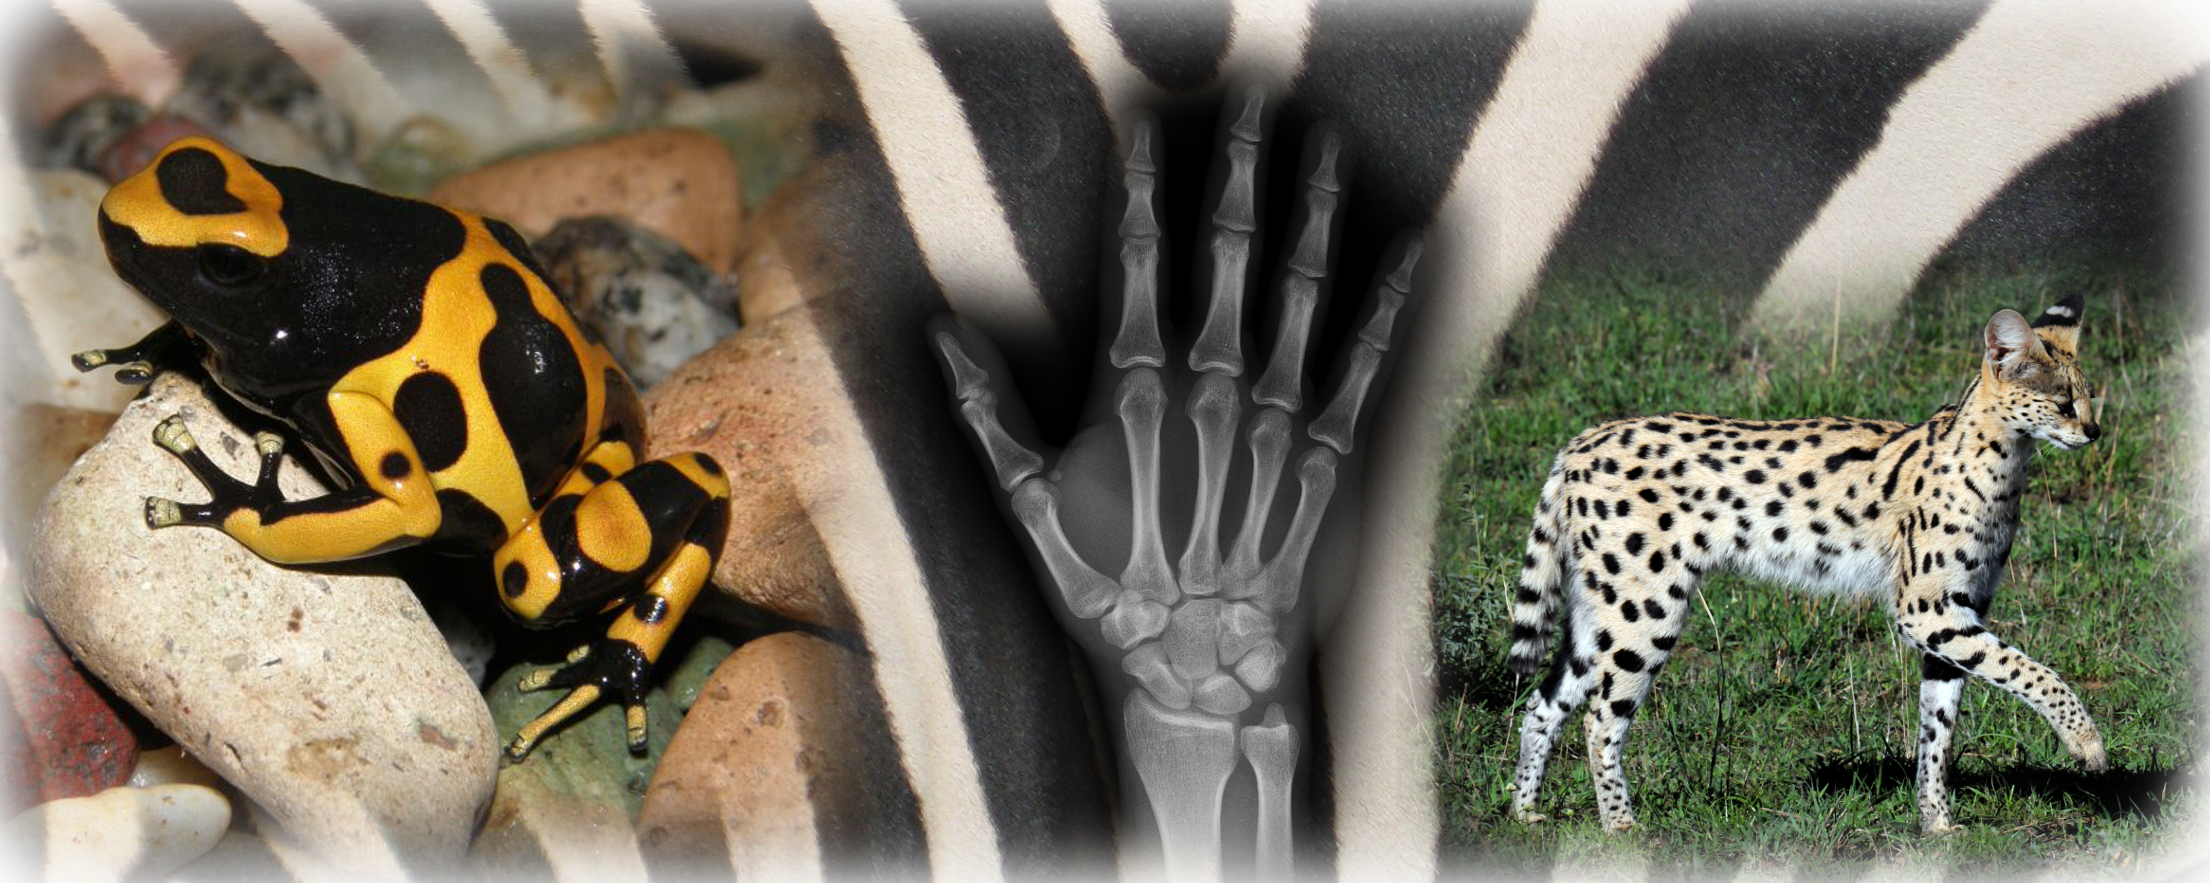
\includegraphics[width=\textwidth]{../Pictures/Feathered_composite.png}
\caption{Examples of spatial patterning. \label{Pattern_examples}}
\end{figure}
\begin{defin}
Patterns are stable, time-independent, spatially heterogeneous density profiles.
\end{defin}
\begin{defin}
Morphogens are pattern forming agents. They can be proteins, cells, animals, etc.
\end{defin}

\section{French flag patterning}
One of the most common mechanisms of pattern creation is that of using cells to read local concentrations of morphogens. If all cells sense the same concentration then they will all differentiate to be the same type of cell. However, if there is a heterogeneous spread of morphogen then we can define thresholds, $T_1>T_2$ such that cells that sense a morphogen level greater than $T_1$ will differentiate differently to those that sense a morphogen amount lower than $T_2$ \see{French flag schematic}. The question thus becomes, how does one generate a heterogeneous morphogen profile?
\begin{figure}[!!!h!!!tb]
\centering
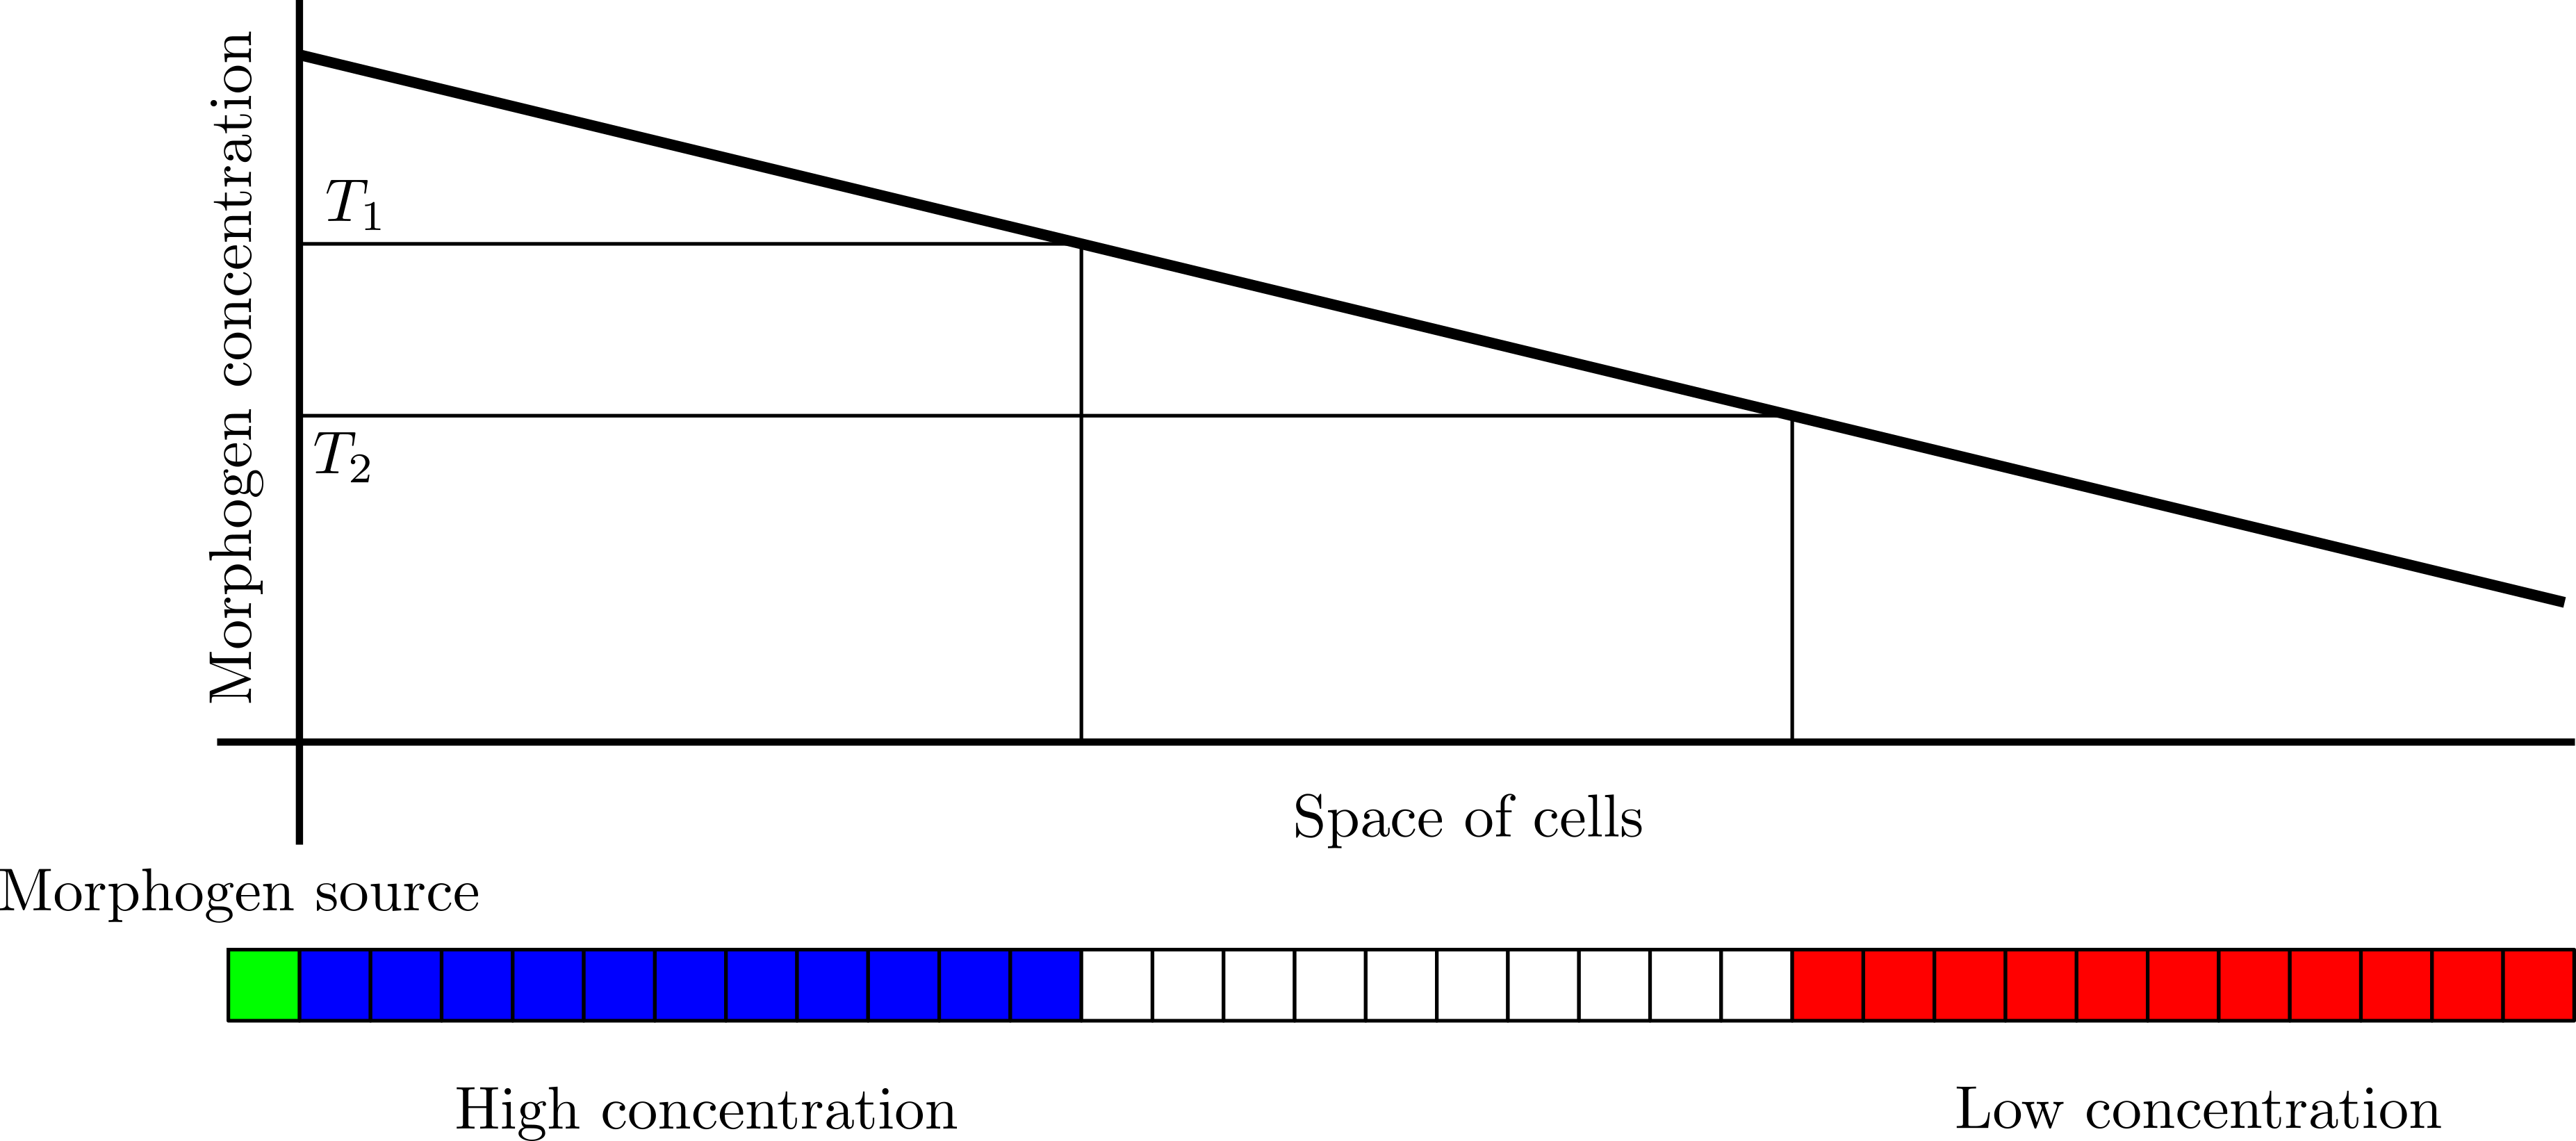
\includegraphics[width=\textwidth]{../Pictures/French_flag_patterning.png}
\caption{Schematic mechanism of French flag patterning. \label{French flag schematic}}
\end{figure}

One of the simplest methods of producing a heterogeneous morphogen profiles is to have heterogeneous production of morphogen. In this section, we will consider isolated regions of production and consider the morphogen pattern that arise. This is known as French flag patterning \see{French flag schematic}.
\begin{example}[frametitle=Localised source]
Consider a morphogen $u$ produced at $x=0$. The morphogen is able to diffuse into the one-dimensional tissue interval $[0,L]$, with diffusion rate $D$. We assume further that the morphogen cannot leave through the boundary $x=L$, \ie it is a reflective boundary. Further, assume that as the morphogen travels it decays at a rate proportional to itself. The mathematical model of this situation is
\bb
\D{u}{t}=\underbrace{D\DD{u}{x}}_{\textrm{Diffusion}}-\underbrace{\gamma u,}_{\textrm{Decay}}\label{FF_eqn}
\ee
\bb
\underbrace{u(0,t)=S,}_{\textrm{Dirichlet condition as a boundary source}} \quad\underbrace{\D{u}{x}(L,t)=0,}_{\textrm{Zero-flux condition at the right-hand side}}
\ee
\bb
\underbrace{u(x,0)=0.}_{\textrm{Initially, there is no morphogen in the field}}\label{FF_IC}
\ee
Note that initial condition do not satisfy the boundary condition. Thus, we expect there would be a singularity in the solution as $t\rightarrow 0$. Although we are able to solve this equation using a separable solution, \ie $u(x,t)=f(x)g(t)$, and Fourier series we are more interested in the steady state situation. Namely, what is the shape of $u$ far into the future?.

\COL{To solve this problem we set $\partial u/\partial t=0$ and solve the resulting ODE problem
\bb
0=D\frac{\rd^2 u}{\rd x^2}-\gamma u,\label{Stationary_gradient}
\ee
\bb
u(0)=S,\quad\frac{\rd u}{\rd x}(L)=0.\label{Boundary_conditions}
\ee}
\COL{We substitute $u=A\exp(\lambda x)$ into \eqns{Stationary_gradient}{Boundary_conditions} where we use $A$ to satisfy the boundary conditions and derive an auxiliary equation for $\lambda$,
\bb
\lambda_{\pm}=\sqrt{\frac{\gamma}{D}}.
\ee
Thus, there are two consistent values of $\lambda$. We could now continue to solve the boundary conditions in terms of
\bb
u=A_+\exp\l x\sqrt{\frac{\gamma}{D}}\r+A_-\exp\l-x\sqrt{\frac{\gamma}{D}}\r,
\ee
however, it is easier to note that
\begin{align}
\cosh(\theta)=&\frac{1}{2}\l\exp\l\theta\r+\exp(-\theta)\r,\\
\sinh(\theta)=&\frac{1}{2}\l\exp\l\theta\r-\exp(-\theta)\r,
\end{align}
and solve in terms of
\bb
u=A\cosh\l x\sqrt{\frac{\gamma}{D}}\r+B\sinh\l x\sqrt{\frac{\gamma}{D}}\r\label{u_hyper}.
\ee
The Dirichlet boundary condition at $x=0$ means that $A=S$ and the zero-flux condition means that $B$ must satisfy
\bb
0=S\sinh\l L\sqrt{\frac{\gamma}{D}}\r+B\cosh\l L\sqrt{\frac{\gamma}{D}}\r.\label{Boundary_B}
\ee
We can rearrange \eqn{Boundary_B} and substitute the form of $B$ back into \eqn{u_hyper} to produce
\bb
u=S\cosh\l x\sqrt{\frac{\gamma}{D}}\r-\frac{S\sinh\l L\sqrt{\frac{\gamma}{D}}\r}{\cosh\l L\sqrt{\frac{\gamma}{D}}\r}\sinh\l x\sqrt{\frac{\gamma}{D}}\r.
\ee}
\end{example}
\begin{figure}[!!!h!!!tb]
\centering
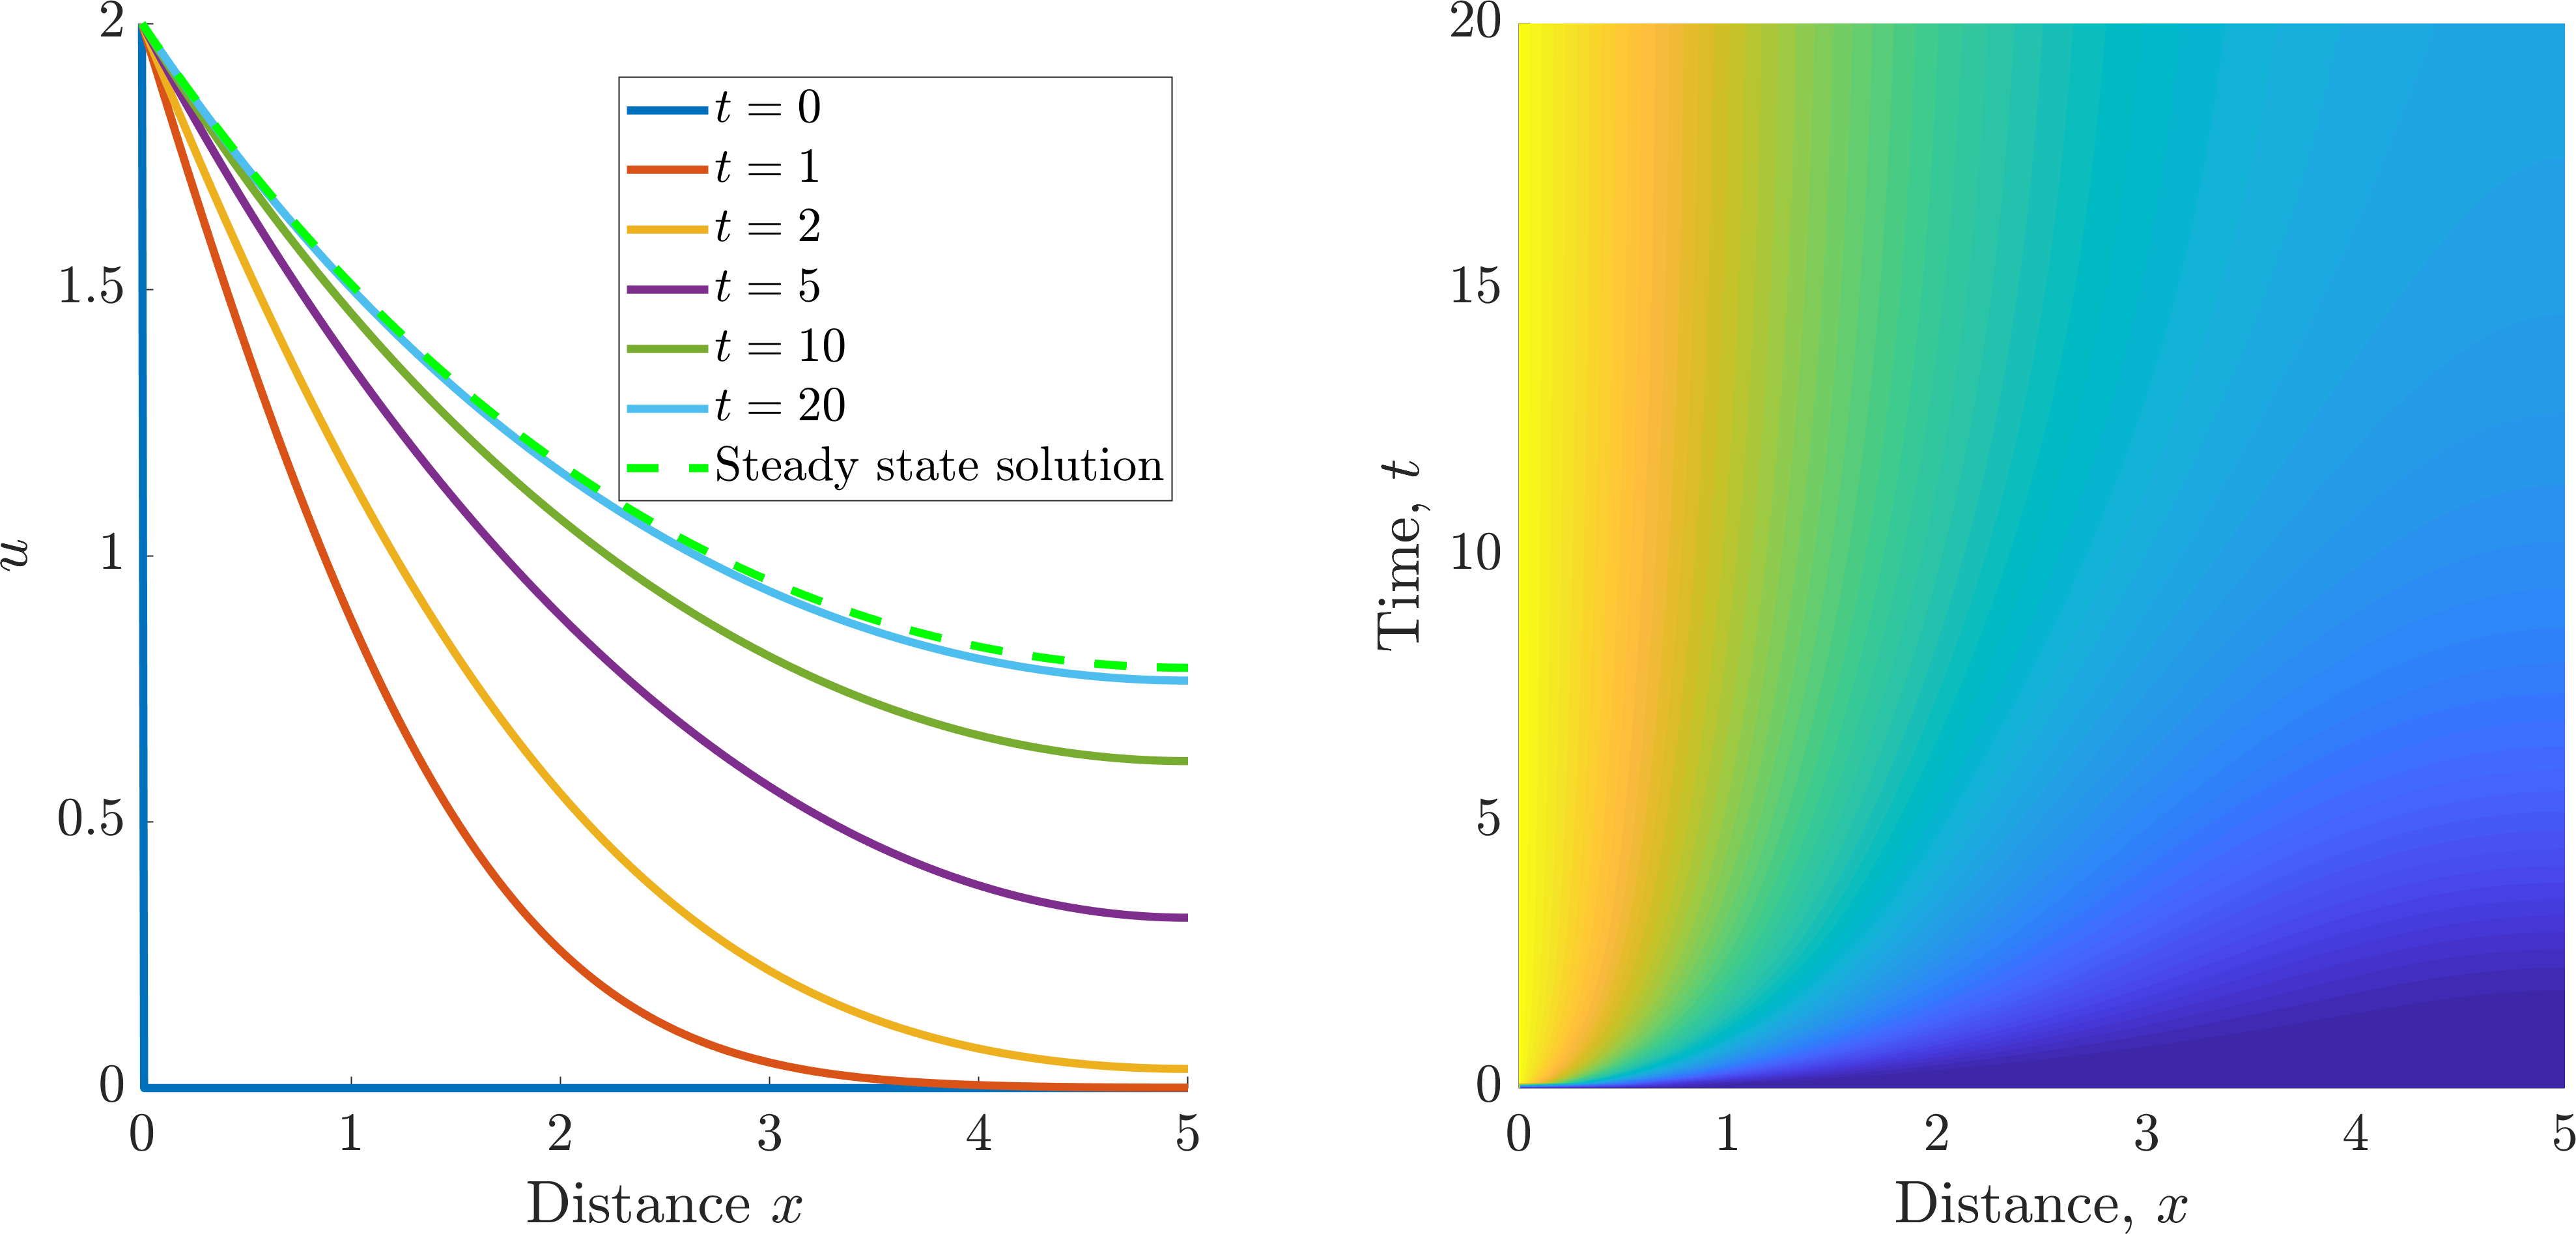
\includegraphics[width=\tp]{../Pictures/French_flag_sims.png}
\caption{Simulation of \eqns{FF_eqn}{FF_IC}. Parameters $L=5, D=1 ,\gamma=0.1$ and $S=2$.\label{French flag sims}}
\end{figure}



\subsection{Digit specification in the limb bud}
One successful applications of the French flag model is in understanding chick limb development \see{Limb_bud}. Biologists have identified a region, called the ``polarising zone''. This small region of cells exists towards the posterior of the chick limb bud and is a localised source of a protein called ``Sonic Hedgehog''\footnote{It is called Sonic Hedgehog because it was originally discovered in flies and upregulating the protein caused the flies to be covered with stiff hair spikes.}, or Shh for short.
\begin{figure}[!!!h!!!tbp]
\centering
\subfigure[\label{Limb_bud_image}\href{https://www.swarthmore.edu/NatSci/sgilber1/DB_lab/Chick/Chick_web_pages/Lauren_Fety/chick_web.html}{A stage 26 chick foetus}]{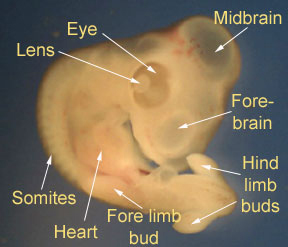
\includegraphics[width=0.3\textwidth]{../Pictures/Limb_bud_image.jpg}}\\
\subfigure[\href{Vargas, Alexander & Kohlsdorf, Tiana & Fallon, John & Vandenbrooks, John & Wagner, Gunter. (2008). The Evolution of HoxD-11 Expression in the Bird Wing: Insights from Alligator mississippiensis. PloS one. 3. e3325. 10.1371/journal.pone.0003325.}{Forelimb bud developing digits.}\label{Gallus_chicken_forelimb_development}]{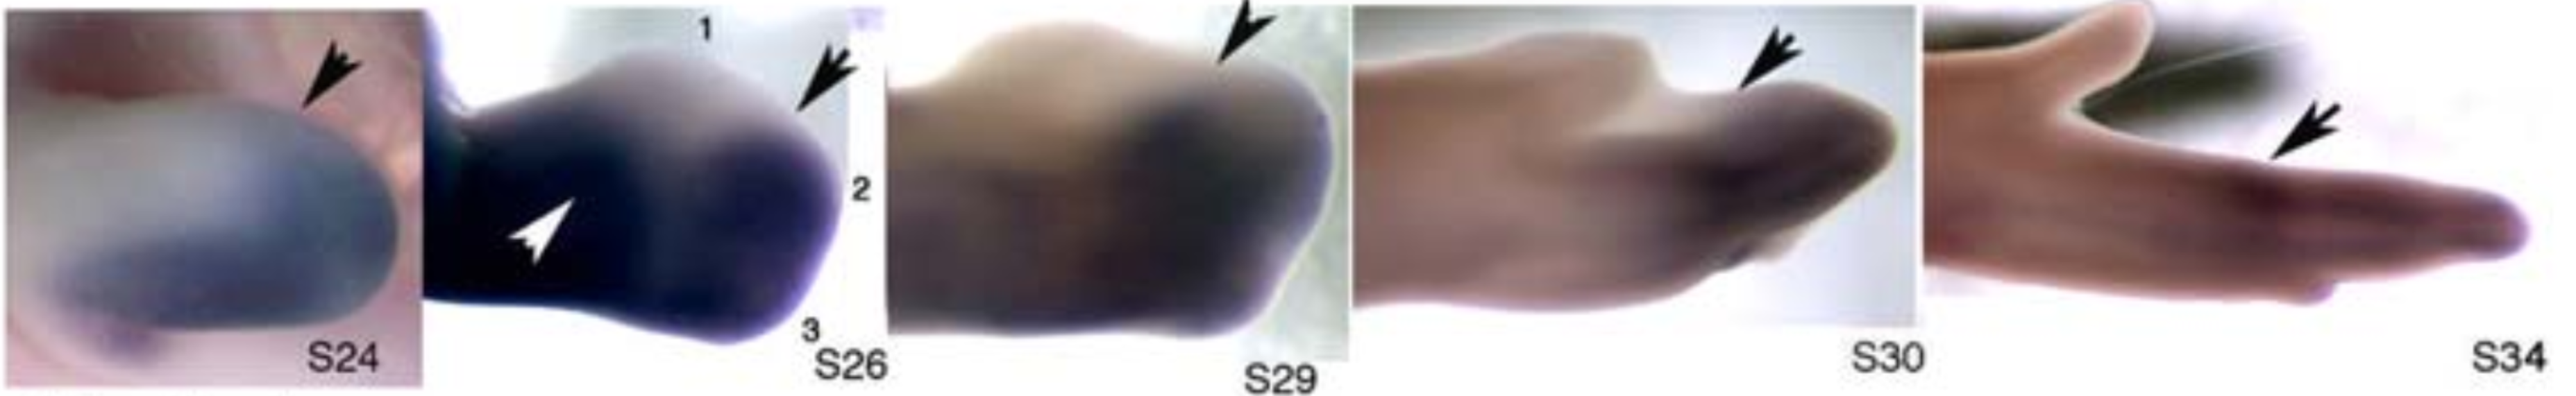
\includegraphics[width=0.8\textwidth]{../Pictures/Gallus_chicken_forelimb_development.png}}
\subfigure[\href{http://www.mun.ca/biology/desmid/brian/BIOL3530/DEVO_11/ch11f12.jpg}{Control and altered digit development by adding exogenous Shh sources.}\label{Digit_specification}]{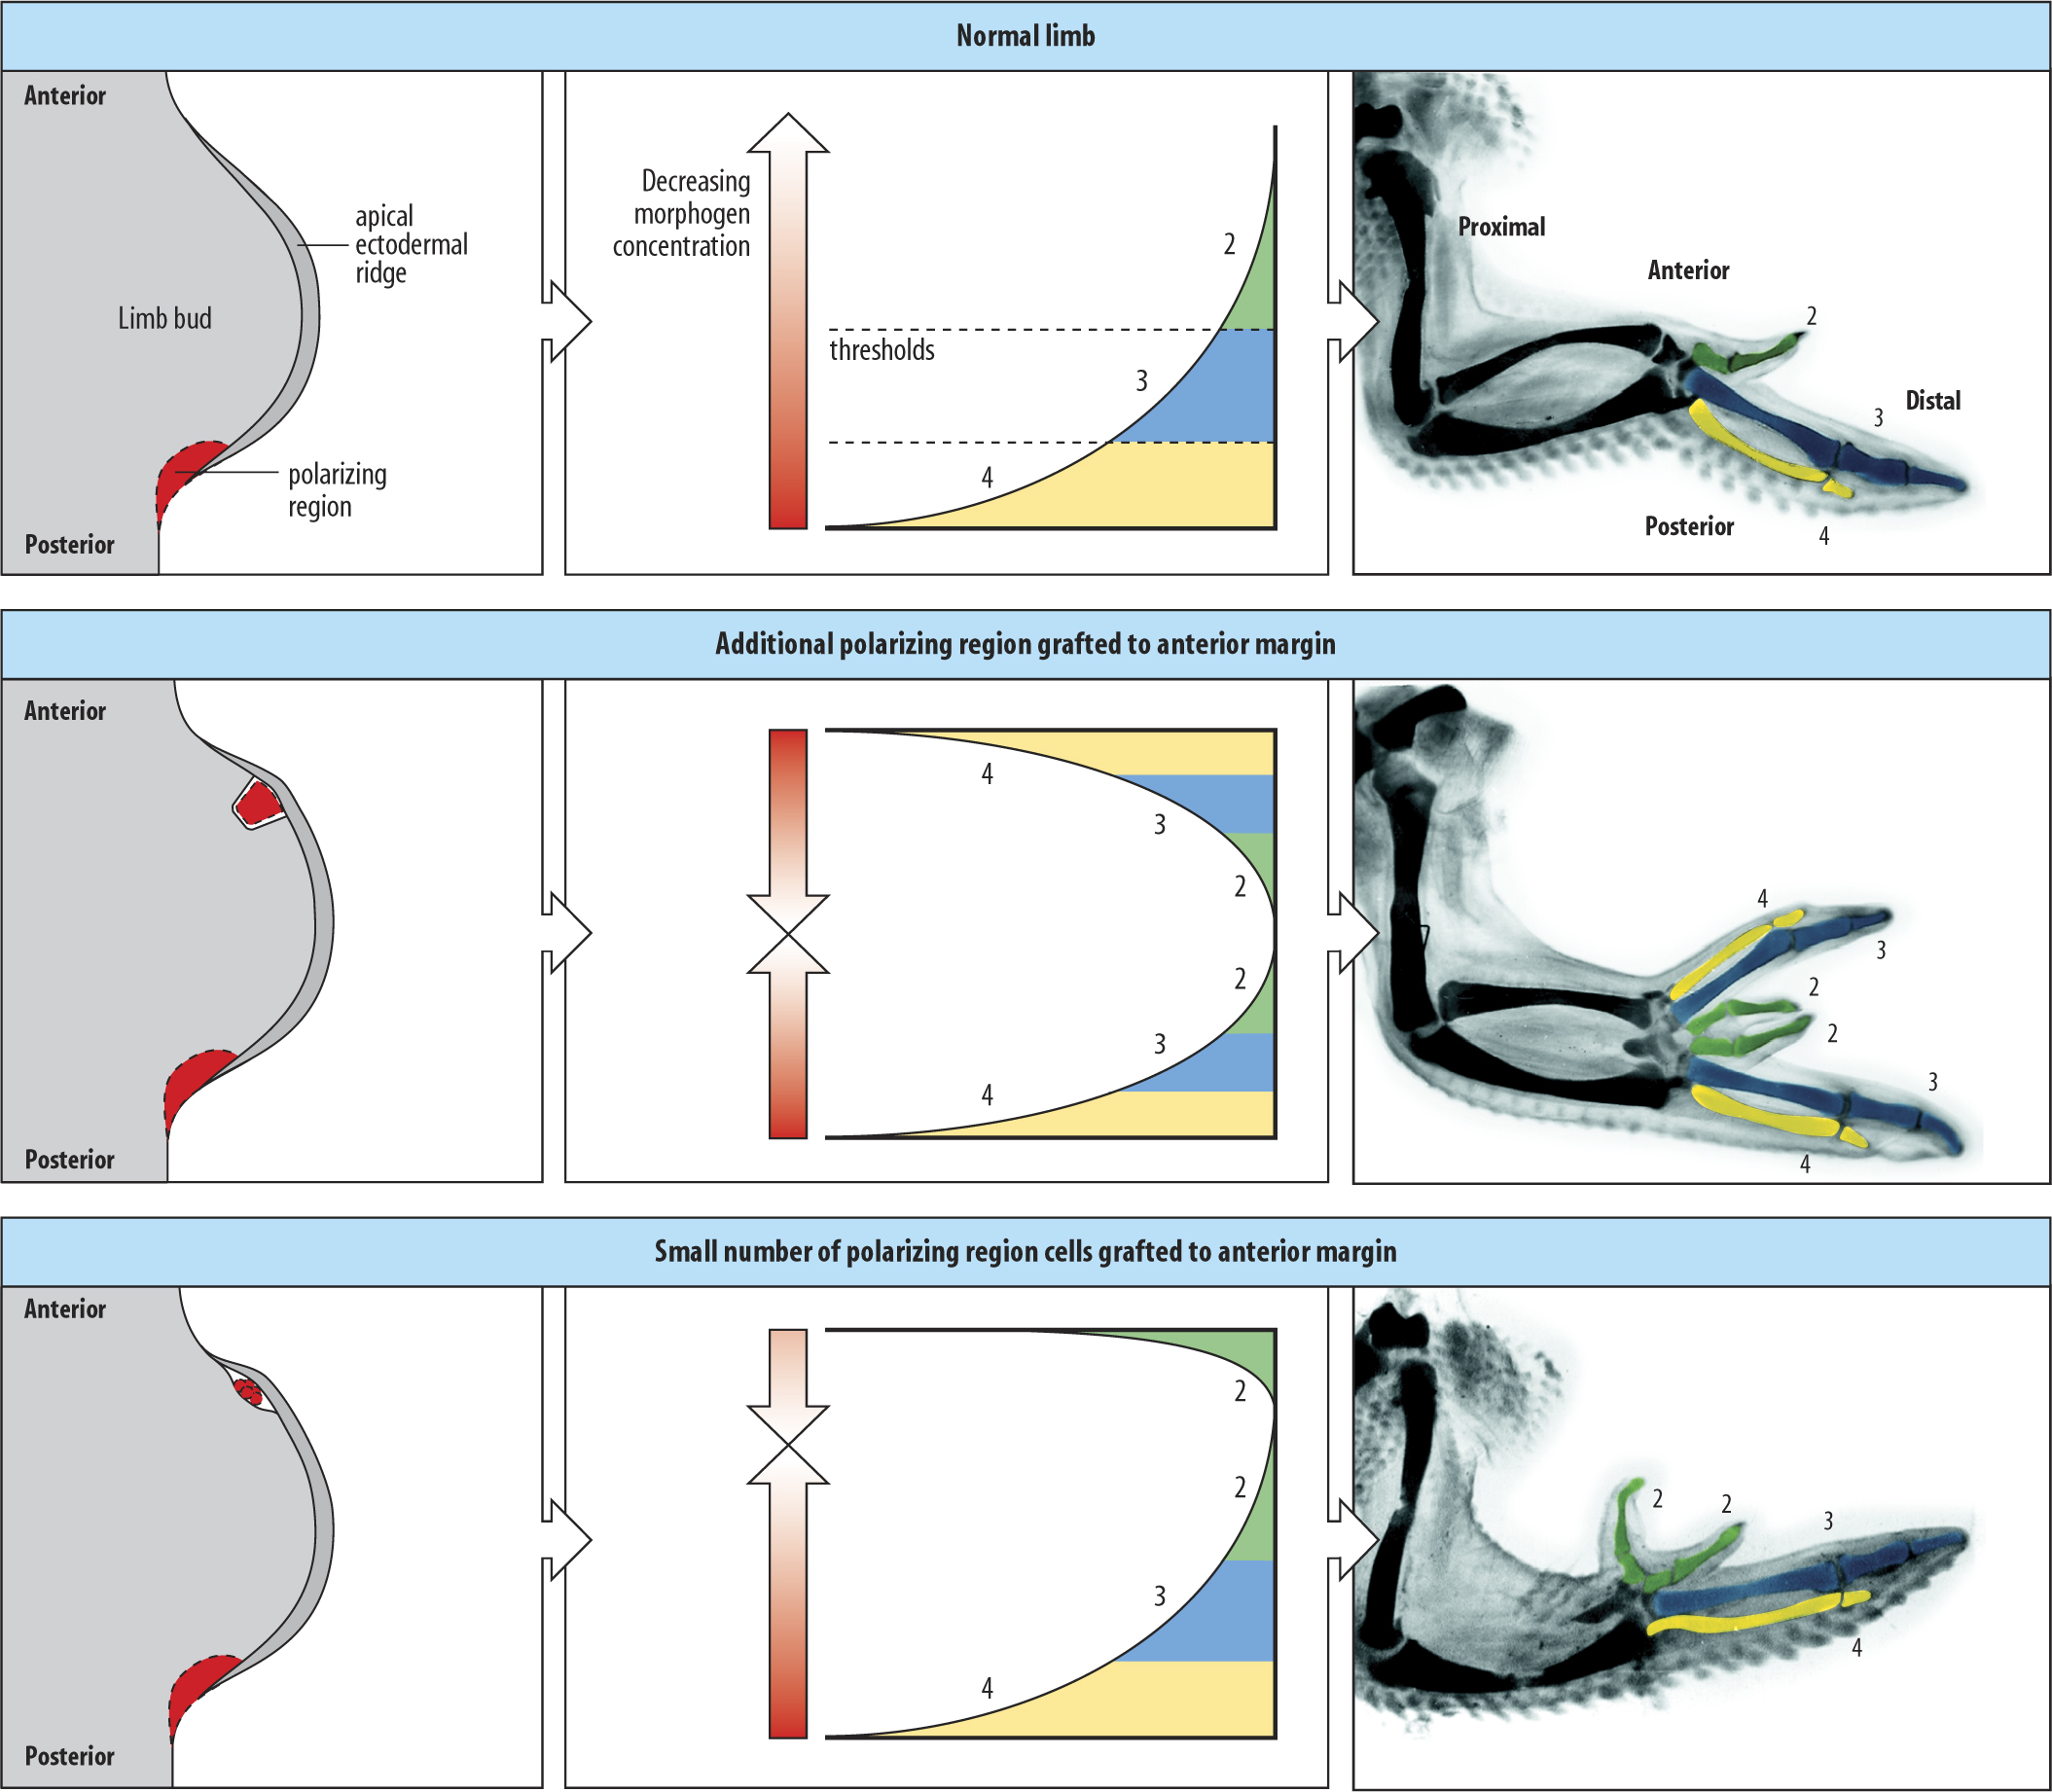
\includegraphics[width=0.8\textwidth]{../Pictures/Digit_specification.jpg}}
\caption{Digit development in chickens. See subcaptions for details. In (b) The arrows highlight Hox genes. The ``S'' numbers refer to the stage of development. You do not need to know these. Note each subcaption is a link to its source.\label{Limb_bud}}
\end{figure}

Shh diffuses out from the polarising zone and appears to specify digit formation through a concentration dependent mechanism. Critically, to really cement the idea that the digits are specified through a French flag mechanism biologists perturbed the limb bud system by adding a second polarising region to the anterior part of the limb bud \see{Digit_specification}. The experimental system gave rise to chicks with extra digits, but, more importantly, the digit identities were reversed. Such results are predicted exactly by adding a second boundary source to \eqn{FF_eqn}. Further, if the second source has a reduced strength then, as we would expect from a concentration dependent, development the extra development never forms the digits that require the highest levels of Shh.

Of course, this is not the end of the story. More recent work in this area suggests that digit specification is not only dependent on the spatial concentration of Shh that the cells sense, but also the amount of time which they are able to sense the concentration. Thus, a high concentration of Shh causes the first digit to develop. However, if we remove the high concentration too early we are left we a digit that is more akin to the final digit that develops.

What you should take from this is that although we have many tools to understand parts of biological development we still do not fully understand the whole. An idea that nicely transitions us to the next section, where understanding each mechanism separately does not provide an undestanding of the whole.

\section{The Turing instability}
Although the French flag mechanism is able to produce long-range patterns it still requires heterogeneity to be built into the system.  We now consider a patterning mechanism that can produce spatial structure from randomness.

In 1952, the logician, computer scientist, code breaker and mathematician Alan Turing proposed a novel mathematical model for pattern formation. He hypothesised that the patterns we see arise due to cells responding to underlying {\it pre-patterns} of chemical concentrations. He termed these chemicals {\it morphogens}, and showed that spatially heterogeneous patterns could arise in systems in which these chemicals reacted with each other and also underwent diffusion - a phenomenon termed {\it diffusion-driven instability}. Making the further assumption that cell fate was determined in a morphogen concentration-dependent manner, the chemical pre-pattern would manifest itself in a pattern composed of spatially heterogeneous cell fates. 

\subsection{Diffusion Driven Instability}
Consider a system of two morphogens $(u,v)$ that are able to interact with each other through kinetics $(f(u,v),g(u,v))$ and diffuse throughout a one-dimensional domain, $[0,L]$, with diffusion coefficients $(D_u,D_v)$, respectively. Finally, we assume that the domain has zero-flux boundary conditions. The mathematical system representing this set up is 
\begin{align}
&\D{u}{t} = D_u\DD{u}{x} + f(u,v),\label{RDu}\\
&\D{v}{t} = D_v\DD{v}{x} + g(u,v),\label{RDv}\\
&\D{u}{x}(x,t)=0 \textrm{ at } x=0,L.\label{BCs}
\end{align}

\begin{defin}
A homogeneous steady state, $(u_s,v_s)$, is a solution satisfying \eqnto{RDu}{BCs} assuming no spatial, or temporal, variation, \ie
\bb
\D{u}{t}=\D{v}{t}=\DD{u}{x}=\DD{v}{x}=0.
\ee
\end{defin}

Using the above definition a homogeneous steady state satisfies
\bb
f(u_s,v_s)=0=g(u_s,v_s).
\ee
We will be looking for conditions under which these states evolve into patterns.
\begin{defin}\label{DDI} A diffusion driven instability, also referred to as a Turing instability, occurs when a homegeneous steady state, which is stable in the absence of diffusion, becomes unstable when diffusion is present.
\end{defin}
The fact that diffusion is going to be responsible for the patterning we are considering is quite surprising. Diffusion, in isolation, disperses a pattern; yet diffusion, in combination with the kinetic terms, can drive a system towards a state with spatial structure.

\subsubsection{A note on initial conditions}
To fully close the system we need to specify initial conditions, $(u(x,0),v(x,0))$, however, these are unimportant and we will be simply assuming that the are random perturbations around the homogeneous steady state.

In a full simulation the final pattern will heavily rely on the initial conditions. Since we are assuming that there is no intelligence behind the pattern construction, these patterns are best suited to understanding individualised pattern, \eg finger prints, zebra stripes, etc.

Equally, due to subcritical bifurcations of the patterning structures it could be possible for the initial conditions to dictate whether patterns are seen, or not. However, such subleties outside of this course.


\subsubsection{A note on boundary conditions}
A homogeneous steady state requires the solution to be uniform across the entire domain. In other words the concentration profile will be flat, or
\bb
\D{u}{x}=0=\D{v}{x}
\ee
everywhere. We note that the homogenous Neumann boundary conditions easily satisfy such requirments. Alternatively, we could use Dirichlet boundary conditions, however, we could have to be careful as to how we fix the boundary values. Namely, we would require that the boundaries are compatible with the homogeneous steady states,
\bb
u(0,t)=u_s=u(L,t)\quad v(0,t)=v_s=v(L,t).
\ee

\subsection{Stability without diffusion}\label{Stability without diffusion}
\COL{As mentioned in definition \ref{DDI} the diffusion driven instabilty requires us to fulfil two properties. Namely, $(u_s,v_s)$ is stable when diffusion is not considered and unstable when diffusion is considered.

In the absence of diffusion \eqns{RDu}{RDv} break down to a system of coupled ODEs, thus, we already know how to derive the stability conditions in this case. Namely, we consider a temporal perturbation to the steady states, \ie
\bb
\l\begin{array}{c}
u\\
v
\end{array}\r
=
\l\begin{array}{c}
u_s\\
v_s
\end{array}\r
+
\l\begin{array}{c}
\epsilon_u\\
\epsilon_v
\end{array}\r\exp(\lambda t),
\ee
where $(\epsilon_u,\epsilon_v)$ is a constant vector and we seek conditions under which Re$(\lambda)<0$. Thus, for $(u_s,v_s)$ to be a stable steady state of
\begin{align}
&\D{u}{t}=f(u,v),\\
&\D{v}{t}=g(u,v),
\end{align}
we consider the eigenvalues of the accompanying Jacobian,
\bb
\bm{J}=\left[ \begin{array}{cc}\noalign{\medskip} f_u&f_v\\
g_u&g_v
\end {array} \right],
\ee
evaluated at the steady state. The eigenvalues, $\lambda$, are solutions to the auxiliary equation
\bb
0=\det(\bm{J}-\lambda I)=\left| \begin{array}{cc}\noalign{\medskip} f_u-\lambda &f_v\\
g_u&g_v-\lambda
\end {array} \right|=\lambda^2-\lambda(f_u+g_v)+f_ug_v-f_vg_u=\lambda^2-\lambda T+D.
\ee
From \app{Characterising the stability of a two-dimensional ODE system} we see that for stability we require
\begin{align}
&T=f_u+g_v<0,\label{T1}\\
&D=f_ug_v-f_vg_u>0.\label{T2}
\end{align}
Equations \eqref{T1} and \eqref{T2} are the first two Turing conditions}

\subsection{Instability with diffusion}
\COL{Now that we are including diffusion we require the steady state perturbation to have a spatial component
\bb
\l\begin{array}{c}
u\\
v
\end{array}\r
=
\l\begin{array}{c}
u_s\\
v_s
\end{array}\r
+
\l\begin{array}{c}
\epsilon_u(x)\\
\epsilon_v(x)
\end{array}\r\exp(\lambda t),\label{Solution_form}
\ee
and that in this case we derive conditions under which $\lambda>0$. Substituting solution form \eqref{Solution_form} into \eqns{RDu}{RDv} gives
\bb
\lambda\exp(\lambda t) \l \begin{array}{c} \epsilon_u\\
\epsilon_v
\end {array} \r
=
\exp(\lambda t)\l\begin{array}{cc} D_u & 0\\
0&D_v
\end {array} \r
\DD{}{x}\l\begin{array}{c}\epsilon_u\\
\epsilon_v
\end {array} \r
+
\l\begin{array}{c}f(u,v)\\
g(u,v)
\end {array} \r,
\ee
where we have suppressed the arguments of $f$ and $g$ for brevity. Assuming that the perturbation is initially small we can expand the $f$ and $g$ terms. As normal, the constant term disappears because $(u_s,v_s)$ is defined to be a homogeneous steady state, so to first order in $\epsilon_u$ and $\epsilon_v$ we have
\bb
\lambda\exp(\lambda t) \l \begin{array}{c} \epsilon_u\\
\epsilon_v
\end {array} \r
=
\exp(\lambda t)\l\begin{array}{cc} D_u & 0\\
0&D_v
\end {array} \r
\DD{}{x}\l\begin{array}{c}\epsilon_u\\
\epsilon_v
\end {array} \r
+
\exp(\lambda t)\l\begin{array}{cc} f_u & f_v\\
g_u&g_v
\end {array} \r
\l\begin{array}{c}\epsilon_u\\
\epsilon_v
\end {array} \r.
\ee
Cancelling out the $\exp(\lambda t)$ term and rearranging provides
\bb
\bm{0}=
\l\begin{array}{cc} D_u & 0\\
0&D_v
\end {array} \r
\DD{}{x}\l\begin{array}{c}\epsilon_u\\
\epsilon_v
\end {array} \r
+
\l\begin{array}{cc} f_u-\lambda & f_v\\
g_u&g_v-\lambda
\end {array} \r
\l\begin{array}{c}\epsilon_u\\
\epsilon_v
\end {array} \r.\label{Matrix_eqn}
\ee
Searching for inspiration, we let
\bb
\bm{D}=\l\begin{array}{cc} D_u & 0\\
0&D_v
\end {array} \r
\quad \bm{\epsilon}=\l\begin{array}{c} \epsilon_u\\
\epsilon_v
\end {array} \r
\ee
and note that the matrix on the right of \eqn{Matrix_eqn} is just $\bm{J}-\lambda \bm{I}$. Note that we should have expected $\bm{J}-\lambda \bm{I}$ to appear on the right of \eqn{Matrix_eqn} because setting the diffusion rates to zero would have landed us back into the case of the previous section, thus, it is a consistency check that  we should be able to recover $\bm{J}-\lambda\bm{I}$ from \eqn{Matrix_eqn}. Upon substituting the new variables into \eqn{Matrix_eqn} we derive
\bb
\bm{0}=\bm{D}\bm{\epsilon}_{xx}+(\bm{J}-\lambda \bm{I})\bm{\epsilon}.\label{Vector_eqn}
\ee
At this point inspiration strikes and we compare \eqn{Vector_eqn} with an analogous scalar equation. Specifically, the solution to the scalar equation
\bb
0=E_{xx}+kE
 \ee
 is $E(x)=A\cos\l \sqrt{k}x\r +B\sin\l \sqrt{k}x\r$, or $E(x)=A\cosh\l \sqrt{k}x\r+B\sinh\l \sqrt{k}x\r$, depending on the sign of $k$ and $A$ and $B$ are constants used to satisfy the boundary conditions. Critically, since we want to satisfy zero-flux boundary conditions we require $k>0$ so we can use the trigonometric form, rather than the hyperbolic functional form.

Thus, by comparison, we suppose
\bb
\bm{\epsilon}=
\l\begin{array}{c} \epsilon_{u1}\\
\epsilon_{v1}
\end {array} \r\cos(kx)+
\l\begin{array}{c} \epsilon_{u2}\\
\epsilon_{v2}
\end {array} \r\sin(kx),\label{Trig_form}
\ee
where $(\epsilon_{u1},\epsilon_{u2},\epsilon_{v1},\epsilon_{v2})$ are constants that are used to satisfy the boundary conditions. To satisfy zero-flux boundary conditions we require
\bb
\l\begin{array}{c} \epsilon_{u2}\\
\epsilon_{v2}
\end {array} \r=\bm{0} \quad \textrm{ and } k=\frac{n\pi}{L}\label{BC_condition}
\ee
for some integer $n$.
To satisfy Dirichlet boundary conditions we require
\bb
\l\begin{array}{c} \epsilon_{u1}\\
\epsilon_{v1}
\end {array} \r=\bm{0} \quad \textrm{ and } k=\frac{n\pi}{L},
\ee
for some integer $n$. To satisfy Robin boundary conditions we would not be able to set either term to zero, rather we would need all degrees of freedom.

Substituting \eqn{Trig_form} into \eqn{Vector_eqn} provides the following consistency relationship
\bb
\bm{0}=\l -\bm{D}k^2+\bm{J}-\lambda \bm{I}\r \bm{\epsilon}.
\ee
Once again this is a nullvector equation, thus, to have non-trivial solutions we require 
\bb
0=\det\l -\bm{D}k^2+\bm{J}-\lambda \bm{I}\r=\det(\bm{M}-\lambda\bm{I})=\left| \begin{array}{cc} -D_uk^2+f_u-\lambda & f_v\\
g_u & -D_vk^2+g_v-\lambda
\end {array} \right|,
\ee
where $\bm{M}=-\bm{D}k^2+\bm{J}$. Simplifying the system we get
\begin{align}
0=&\l-D_uk^2+f_u-\lambda \r\l-D_uk^2+f_u-\lambda \r-g_uf_v,\nonumber\\
=&\lambda^2 -\lambda \l f_u+g_v-k^2(D_u+Dv)\r+\l-D_uk^2+f_u\r\l-D_vk^2+g_v \r-g_uf_v,\nonumber\\
=&\lambda^2 -\lambda \textrm{trace}(M)+\det(M).\label{Dispersion}
\end{align}

Since we require an instability to occur at least one solution of \eqn{Dispersion} has to have positive real part. Critically, from \eqn{T1} we know that $f_u+g_v<0$, further, since $k^2, D_u$ and $D_v$ are all positive we must have that
\bb
0>f_u+g_v-k^2(D_u+Dv)=\textrm{trace}(M).
\ee
Comparing this with the result in \fig{TD_stability} we see that the only way to get an instability is if $\det(M)<0$, namely
\bb
\det(M)=D_uD_vk^4-k^2(D_vf_u+D_ug_v)+f_ug_v-g_uf_v<0.\label{Det0}
\ee
Since $\det(M)$ is quadratic in $k^2$ then it has a negative region if and only if it has two real roots, $k^2_\pm$, say, \see{Root_schematic}. Solving $\det(M)=0$ provides
\bb
k^2_\pm=\frac{(D_vf_u+D_ug_v)\pm\sqrt{(D_vf_u+D_ug_v)^2-4D_uD_v(f_ug_v-g_uf_v)}}{2D_uD_v},
\ee
for these two roots to be real and positive we require
\begin{align}
D_vf_u+D_ug_v>0, \quad\quad &\textrm{(to ensure that $k^2_->0$)}\label{T3}\\
(D_v+D_u)^2-4D_uD_v(f_ug_v-g_uf_v)>0. \quad\quad &\textrm{(to make the roots real)}\label{T4}
\end{align}
Inequalities \eqref{T3} and \eqref{T4} are the third and fourth Turing conditions.

Satisfying inequalities \eqref{T3} and \eqref{T4} ensures that there are real values $k$, such that $k^2_-<k^2<k^2_+$ for which \eqn{Dispersion} has positive real roots. However, we are not quite done. As a final step we must ensure that our solution satisfies the boundary conditions as specified in \eqn{BC_condition}. Collecting all of these requirements together we generate the full set of Turing conditions,}
\begin{figure}[!!!h!!!tbp]
\centering
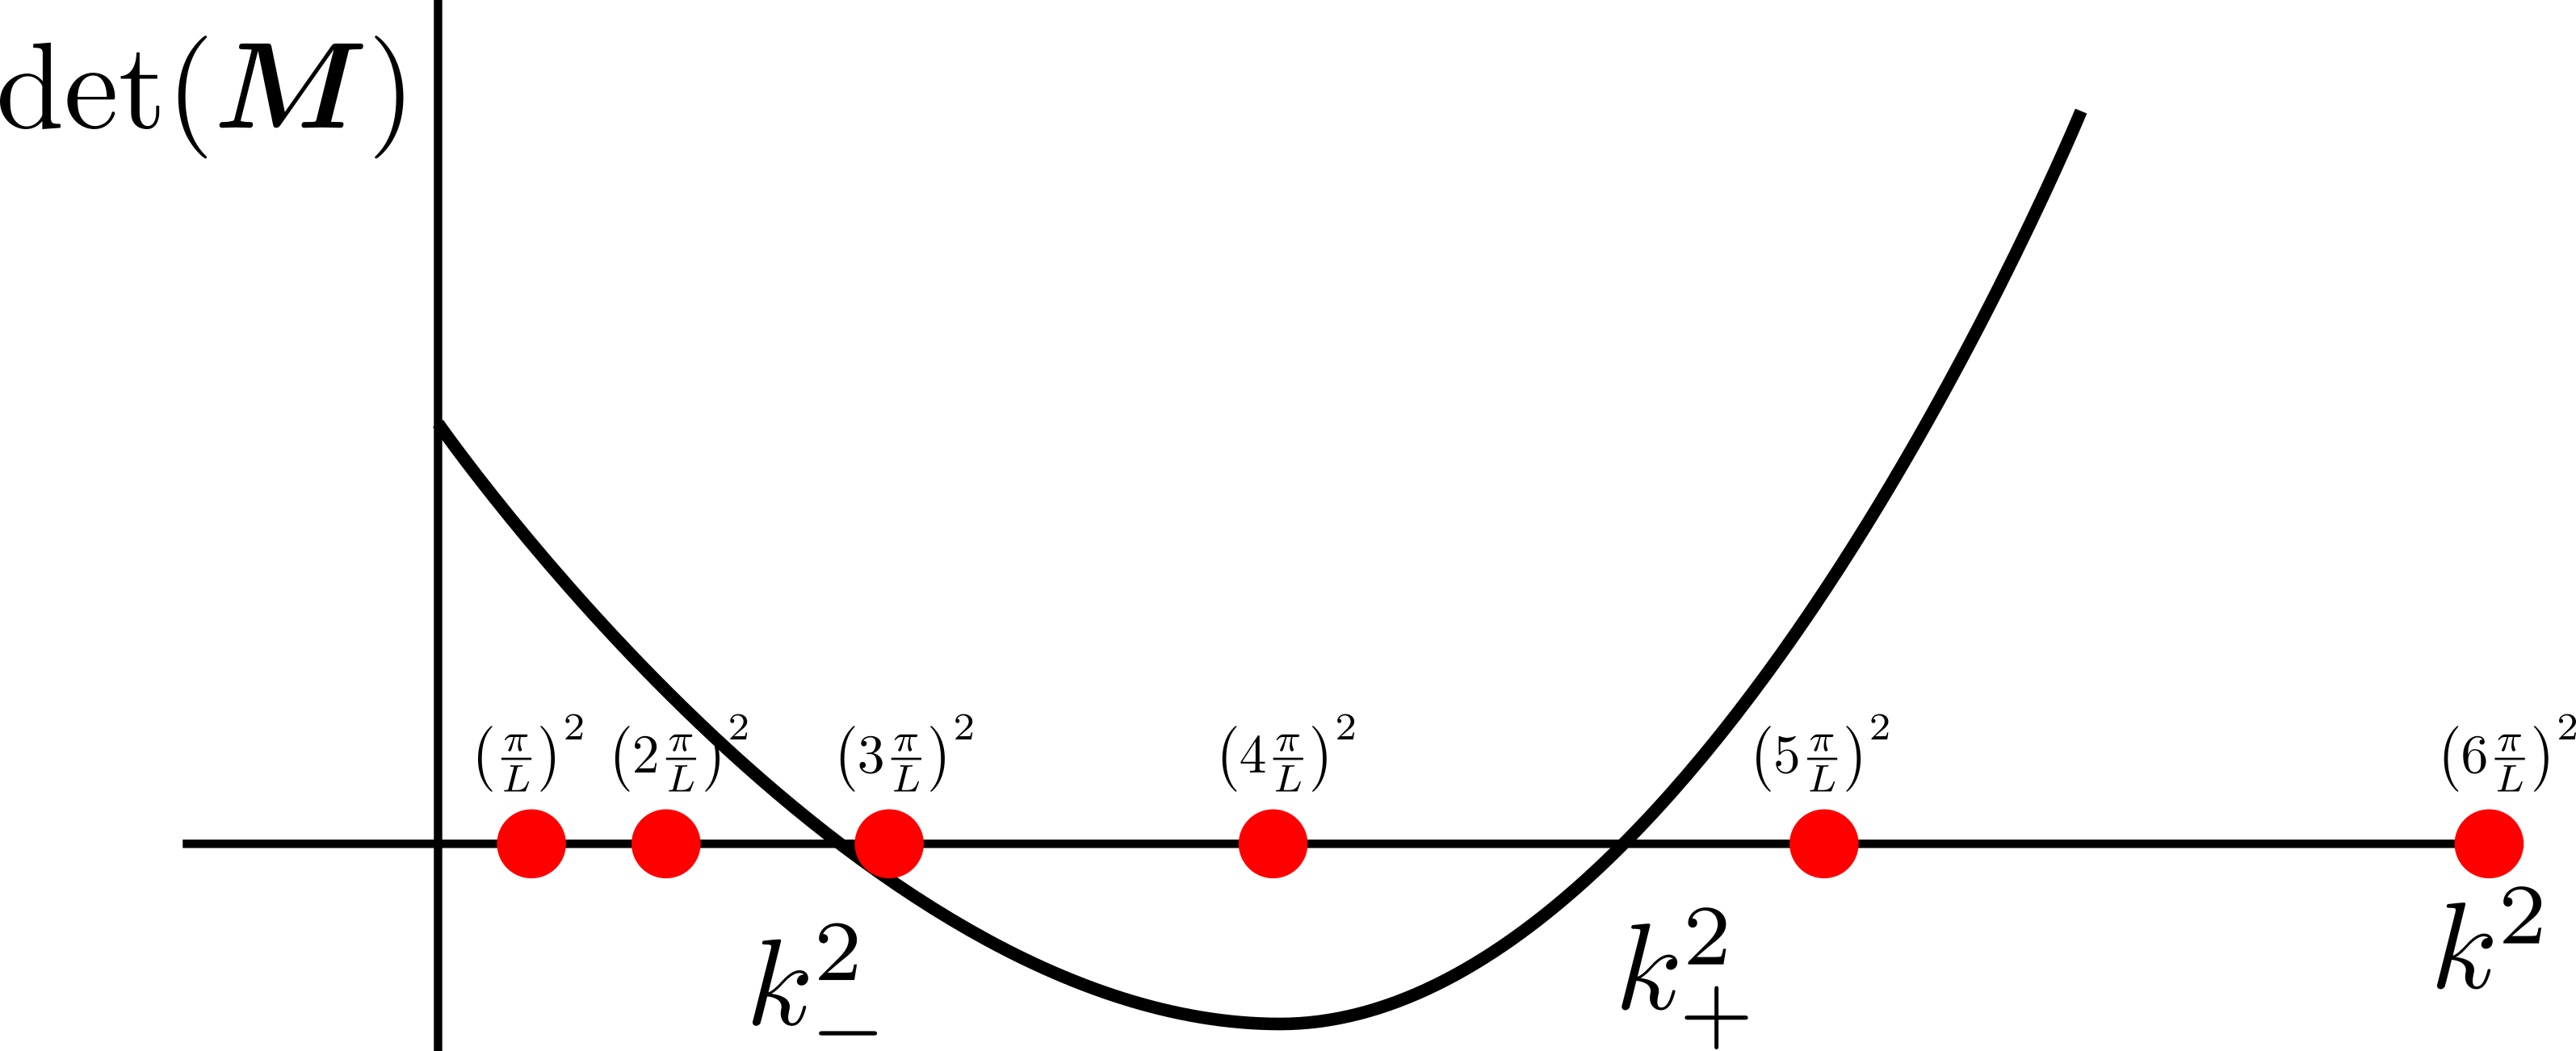
\includegraphics[width=0.8\textwidth]{../Pictures/Root_schematic.png}
\caption{Schematic diagram of $\det(\bm{M})$. \label{Root_schematic}}
\end{figure}


\begin{tcolorbox}

Necessary conditions to produce patterning in using \eqns{RDu}{RDv}

\begin{align}
&f_u+g_v<0,\label{TT1}\\
&f_ug_v-f_vg_u>0,\label{TT2}\\
&D_vf_u+D_ug_v>0,\label{TT3}\\
&(D_vf_u+D_ug_v)^2-4D_uD_v(f_ug_v-g_uf_v)>0,\label{TT4}\\
&\exists n\in \mathbb{Z} \textrm{ such that }k_-<\frac{n\pi}{L}<k_+.\label{TT5}
\end{align}
\end{tcolorbox}

\subsection{Corollaries to Turing's theory}\label{Corollaries}
We have derived a number of necessary conditions that allow patterns to occur. However, considering our results a little further we gain a number of further insights.
\COL{\begin{enumerate}
\item Our derivation only guarantees that the steady state will be stable without diffusion and unstable with diffusion. It does not guarantee that the instability will stabilise again in a patterned form. The stability of the patterned state is governed by the non-linear terms and their analysis is outside of this course. 
\item By comparing inequalities \eqref{TT1} and \eqref{TT3} we produce two conclusions. Firstly, $f_u$ and $g_v$ must be of opposite signs and, secondly, $D_v\neq D_u$. \label{Ds_not_equal}
\item Having concluded that $f_u$ and $g_v$ are opposite signs inequality \eqref{TT2} demonstrates that $f_v$ and $g_u$ must be of opposite sign too.

\item The last two insights constrain the sign forms of the Jacobian to the following four types
\bb
\bm{J}=\l\begin{array}{cc} + & +\\
-&-
\end {array} \r,
\l\begin{array}{cc} - & -\\
+&+
\end {array} \r
,\l\begin{array}{cc} + & -\\
+&-
\end {array} \r,
\l\begin{array}{cc} - & +\\
-&+
\end {array} \r.
\ee
Note that the second and fourth sign structures can be gained from the first and third, respectively, by swapping the definitions of $u$ and $v$.
\item The first two Jacobian forms are known are cross kinetics. They produce patterns that are out of phase with one another. Namely, peak in $u$ correspond to troughs in $v$. The last two are called pure kinetics. They produce patterns that are in phase with one another. Namely, peak in $u$ correspond to peaks in $v$.
\item Consider sign structures 1 and 3. In both cases $f_u>0$ this means that the $u$ population causes an increase in the $u$ population, so $u$ is known as a self-activator. Similarly, because $g_v<0$ this means that $v$ is a self inhibitor.
\item Combining sign structures 1 and 3 with \eqns{TT1}{TT3} means that $D_v>D_u$. Combining this result with the previous definitions of the characteristics of $u$ and $v$ provides us with an intuitive way of understanding patterning. Namely, the system works via \textit{long range inhibition and short range activation}.
\item If the domain length, $L$, is too small then we cannot satisfy inequality \eqref{TT5}. Thus, we see that it is not enough to consider the dynamics occurring over  space; the space has to be big enough to support the patterning wavelength.
\end{enumerate}}


\begin{example}[frametitle=Specific Turing kinetic example: Schnakenberg kinetics]
We consider a spatially extended version of the Schnakenberg kinetics as a model of morphogen populations,
\begin{align}
&\D{u}{t} = \DD{u}{x} + \alpha-u+u^2v,\label{Schnaku}\\
&\D{v}{t} = D_v\DD{v}{x} + \beta-\alpha-u^2v,\label{Schnakv}
\end{align}
on a domain, $[0,L]$ with zero-flux boundary conditions and random perturbation around the steady state as an initial condition. Further, we suppose $D_v, \alpha$ and $\beta$ are positive constants. Derive the Turing conditions that need to be satisfied for a pattern to appear.


\begin{enumerate}
\item \COL{First we need to find the homogeneous steady states from
\begin{align}
&0=\alpha-u+u^2v, \label{Homo_schnak_u}\\
&0=\beta-\alpha-u^2v.\label{Homo_schnak_v}
\end{align}
Solving \eqns{Homo_schnak_u}{Homo_schnak_v} simultaneously we derive
\bb
(u_s,v_s)=\l \beta,\frac{\beta-\alpha}{\beta^2}\label{Schnak_stst}\r.
\ee
Since we want a biologically relevant steady state we require $\beta>\alpha$.}


\item \COL{We now find the Jacobian,
\bb
\bm{J}(u_s,v_s)=\l\begin{array}{cc} -1+2u_sv_s & u_s^2\\
-2u_sv_s&-u_s^2
\end {array} \r.
\ee
As we have seen previously, it is generally easier to not substitute components in until the end. However, we will make a note here that for a Turing instability to occur we must have that the sign structure of the Jacobian corresponds to those shown in Section \ref{Corollaries}. Since the Jacobian structure is currently
\bb
\bm{J}(u_s,v_s)=\l\begin{array}{cc} ? & +\\
-&-
\end {array} \r
\ee
we must have that $f_u>0$, namely
\begin{align}
&0<-1+2u_sv_s,\nonumber\\
\implies &0<-1+2\frac{\beta-\alpha}{\beta},\nonumber\\
\implies &2\alpha<\beta,\nonumber\\
\implies &\alpha<\frac{\beta}{2},\nonumber
\end{align}
which we note is a sharper bound than $\alpha<\beta$ derived above for the steady states.}



\item \COL{Next we compute the trace and determinant of $\bm{J}$ and determine conditions under which the trace is negative and the determinant is positive,
\begin{align}
&0>-1+2u_sv_s-u_s^2,\label{Schnak_trace}\\
&0<(-1+2u_sv_s)(-u_s^2)-(u_s^2)(-2u_sv_s)=u_s^2.\label{Schnak_det}
\end{align}
Inequality \eqref{Schnak_det} is always satisfied, so we only need to satisfy \eqn{Schnak_trace}. Substituting in the values of \eqn{Schnak_stst} we derive
\begin{align}
0>&-\beta^2+2\frac{\beta-\alpha}{\beta}-1,\nonumber\\
\implies \alpha>&\frac{-\beta^3+\beta}{2}=\frac{-\beta(\beta+1)(\beta-1)}{2}.
\end{align}}
\COL{Thus, for the homogeneous steady state to be stable in the absence of diffusion we require
\bb
\frac{\beta}{2}>\alpha>\frac{-\beta(\beta+1)(\beta-1)}{2},
\ee
which is illustrated in \fig{Stable_alpha_region}.}


\item \COL{For pattern formation to occur we now require that the steady state becomes unstable once diffusion is added. We construct
\bb
\bm{M}=
\l\begin{array}{cc} -k^2-1+2u_sv_s & u_s^2\\
-2u_sv_s&-k^2D_v-u_s^2
\end {array} \r.
\ee
and derive conditions under which
\bb
\det(\bm{M})=D_vk^4+(D_v(1-2u_sv_s)+u_s^2)k^2+u_s^2
\ee
is negative for some region of $k^2$. We could use inequalities \eqref{TT3} and \eqref{TT4}, but it is quite informative to solve for $k^2$ and observe where our conditions stem from. Specifically,
\bb
k^2_\pm=\frac{-(D_v(1-2u_sv_s)+u_s^2)\pm\sqrt{(D_v(1-2u_sv_s)+u_s^2)^2-4D_vu_s^2}}{2D_v},\label{Wave_modes}
\ee
so we require
\bb
0<-(D_v(1-2u_sv_s)+u_s^2)=2D_v\frac{\beta-\alpha}{\beta} -\beta^2-D_v,\nonumber
\ee
\bb
\implies D_v>\frac{\beta^3}{\beta-2\alpha},\label{First_Dv_inequality}
\ee
and
\bb
0<(D_v(1-2uv)+u^2)^2-4D_vu^2\nonumber
\ee
\bb
\implies 0 < (\beta-2\alpha)^2D_v^2-2\beta^3(3\beta-2\alpha)D_v+\beta^6=h(D_v)\label{Dv_inequality}
\ee
The function $h(D_v)$ is a positive quadratic in $D_v$, so it is satisfiable for large enough $D_v$. Equally, we notice that since $\alpha<\beta/2<3\beta/2$ the coefficient of $D_v$ is negative. We complete the square of \eqn{Dv_inequality} to derive that we require
\bb
0<\l D_v-\frac{\beta^3(3\beta-2\alpha)}{(\beta-2\alpha)^2}\r^2+\frac{\beta^6}{(\beta-2\alpha)^2}-\l\frac{\beta^3(3\beta-2\alpha)}{(\beta-2\alpha)^2}\r^2.
\ee
In this form we see that the minimum value of the parabola (with respect to $D_v$) is
\bb
\frac{\beta^6}{(\beta-2\alpha)^2}-\l\frac{\beta^3(3\beta-2\alpha)}{(\beta-2\alpha)^2}\r^2.
\ee
Thus, if the minimum value is positive then \eqn{Dv_inequality} is always satisfied. Namely
\begin{align}
&0<\frac{\beta^6}{(\beta-2\alpha)^2}-\l\frac{\beta^3(3\beta-2\alpha)}{(\beta-2\alpha)^2}\r^2,\nonumber\\
\implies &(3\beta-2\alpha)^2<(\beta-2\alpha)^2
\end{align}}
\COL{which is impossible because $0<\beta-2\alpha<3\beta-2\alpha$. Thus, $h(D_v)$ must have two roots
\bb
D_{\pm v}=\frac{\beta^3(3\beta-2\alpha)\pm\beta^3\sqrt{(3\beta-2\alpha)^2-(\beta-2\alpha)^2}}{(\beta-2\alpha)^2}\label{Dv_root}
\ee
and inequality \eqref{Dv_inequality} will be satisfied for  $D<D_{-v}$ and $D>D_{+v}$. Rearranging \eqn{Dv_root} to
\begin{align}
D_{\pm v}=&\frac{\beta^3}{(\beta-2\alpha)}\l \l 1+\frac{2\beta}{(\beta-2\alpha)}\r\pm\sqrt{\l 1+\frac{2\beta}{(\beta-2\alpha)}\r^2-1}\r,\nonumber\\
=&\frac{\beta^3}{(\beta-2\alpha)}\l \l 1+\frac{2\beta}{(\beta-2\alpha)}\r\pm\sqrt{\l \frac{2\beta}{(\beta-2\alpha)}\r^2+2\frac{2\beta}{(\beta-2\alpha)}}\r.
\end{align}
we can now see that
\begin{align}
1<& \l 1+\frac{2\beta}{(\beta-2\alpha)}\r+\sqrt{\l \frac{2\beta}{(\beta-2\alpha)}\r^2+2\frac{2\beta}{(\beta-2\alpha)}},\nonumber\\
1>& \l 1+\frac{2\beta}{(\beta-2\alpha)}\r-\sqrt{\l \frac{2\beta}{(\beta-2\alpha)}\r^2+2\frac{2\beta}{(\beta-2\alpha)}}.
\end{align}
So,
\bb
D_{+v}>\frac{\beta^3}{\beta-2\alpha}>D_{-v}.
\ee
Hence, from inequality \eqref{First_Dv_inequality} we can never be in the situation that $D_v<D_{-v}$ and we only need to consider $D_v>D_{+v}$ \see{Schnakeberg_diffusion_curve}.}



\item \COL{Finally, we need to ensure that our domain is large enough to support patterning. Namely, we need to ensure that there exists integers, $n$, such that
\bb
k_-<\frac{n\pi}{L}<k_+.
\ee
Note we tend to use the lower limit because this normally allows us to just fine tune what modes are available. Thus we want to satisfy
\bb
\frac{n\pi}{k_+}<L,\label{Critical_length}
\ee
where we note that the smallest $L$ can be is when $n=1$. Substituting \eqn{Wave_modes} into \eqn{Critical_length} we derive that the length of the domain must be at least
\bb
\pi\sqrt{\frac{2D_v}{-(D_v(1-2u_sv_s)+u^2)+\sqrt{(D_v(1-2u_sv_s)+u_s^2)^2-4D_vu_s^2}}}.
\ee}




\item \COL{Collecting all the pertinent inequalities together then for patterning to form we need to }\COL{satisfy:
\begin{align}
&\frac{\beta}{2}>\alpha>\frac{-\beta(\beta+1)(\beta-1)}{2},\label{alpha_ineq}\\
&D_v>\frac{\beta^3}{(\beta-2\alpha)}\l \l 1+\frac{2\beta}{(\beta-2\alpha)}\r\pm\sqrt{\l 1+\frac{2\beta}{(\beta-2\alpha)}\r^2-1}\r,\label{Dv_ineq}\\
&L>\pi\sqrt{\frac{2D_v}{-(D_v(1-2uv)+u^2)+\sqrt{(D_v(1-2uv)+u^2)^2-4D_vu^2}}}.\label{L_ineq}
\end{align}
Taking $D_v$ and $L$ large enough will always allow us to satisfy inequalities \eqref{Dv_ineq} and \eqref{L_ineq}. Choosing $\alpha$ is slightly more tricky. Suppose we fix $\beta=0.9$ then
\bb
0.45>\alpha>0.0855.
\ee
So, let us fix $\alpha=0.1$. Inequality \eqref{Dv_ineq} then becomes
\bb
D_v>7.29,
\ee
so, let $D_v=10$. Finally, inequality \eqref{L_ineq} becomes
\bb
L>4.28,
\ee
so let $L=5$. Simulating the system under these parameter values provides \fig{Schnak_pde}. Clearly, we see although initially there is nothing but noise the system can quickly and easily arrange itself to a heterogeneous solution.}
\end{enumerate}
\end{example}
\begin{figure}[!!!h!!!tbp]
\centering
\subfigure[\label{Stable_alpha_region}]{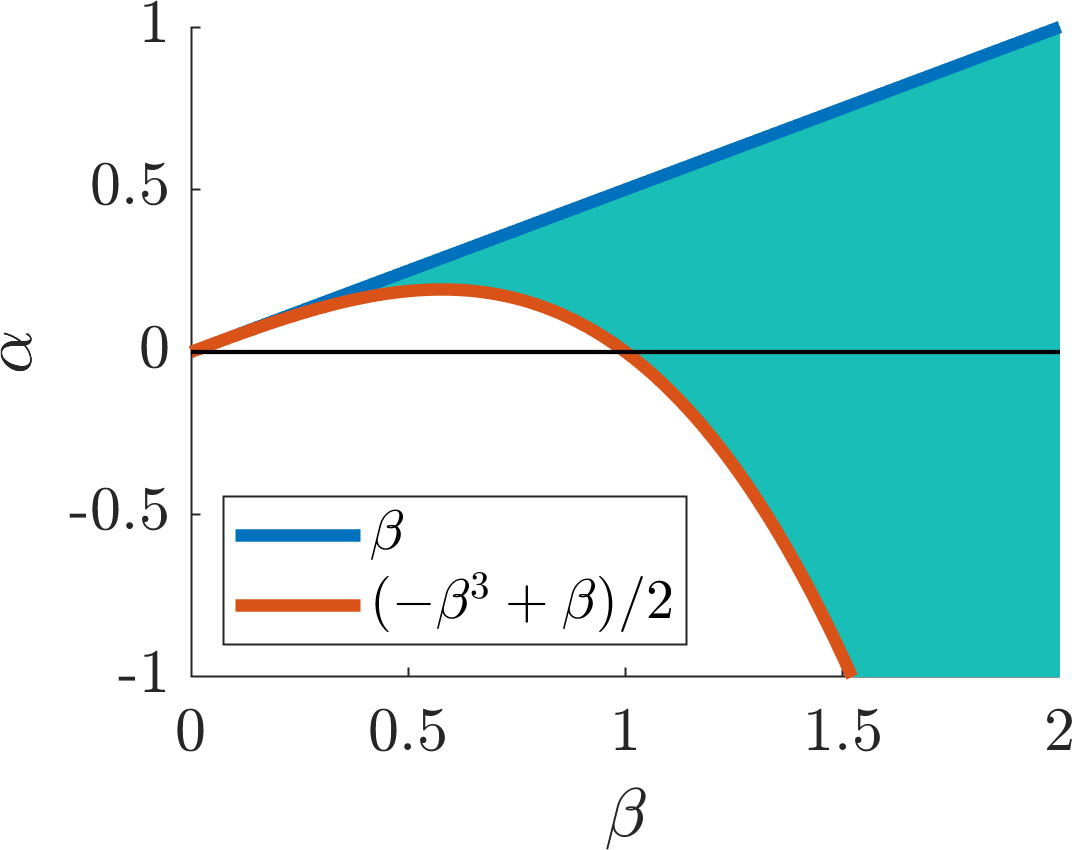
\includegraphics[width=\ttp]{../Pictures/Stable_alpha_region.png}}
\subfigure[\label{Schnakeberg_diffusion_curve}]{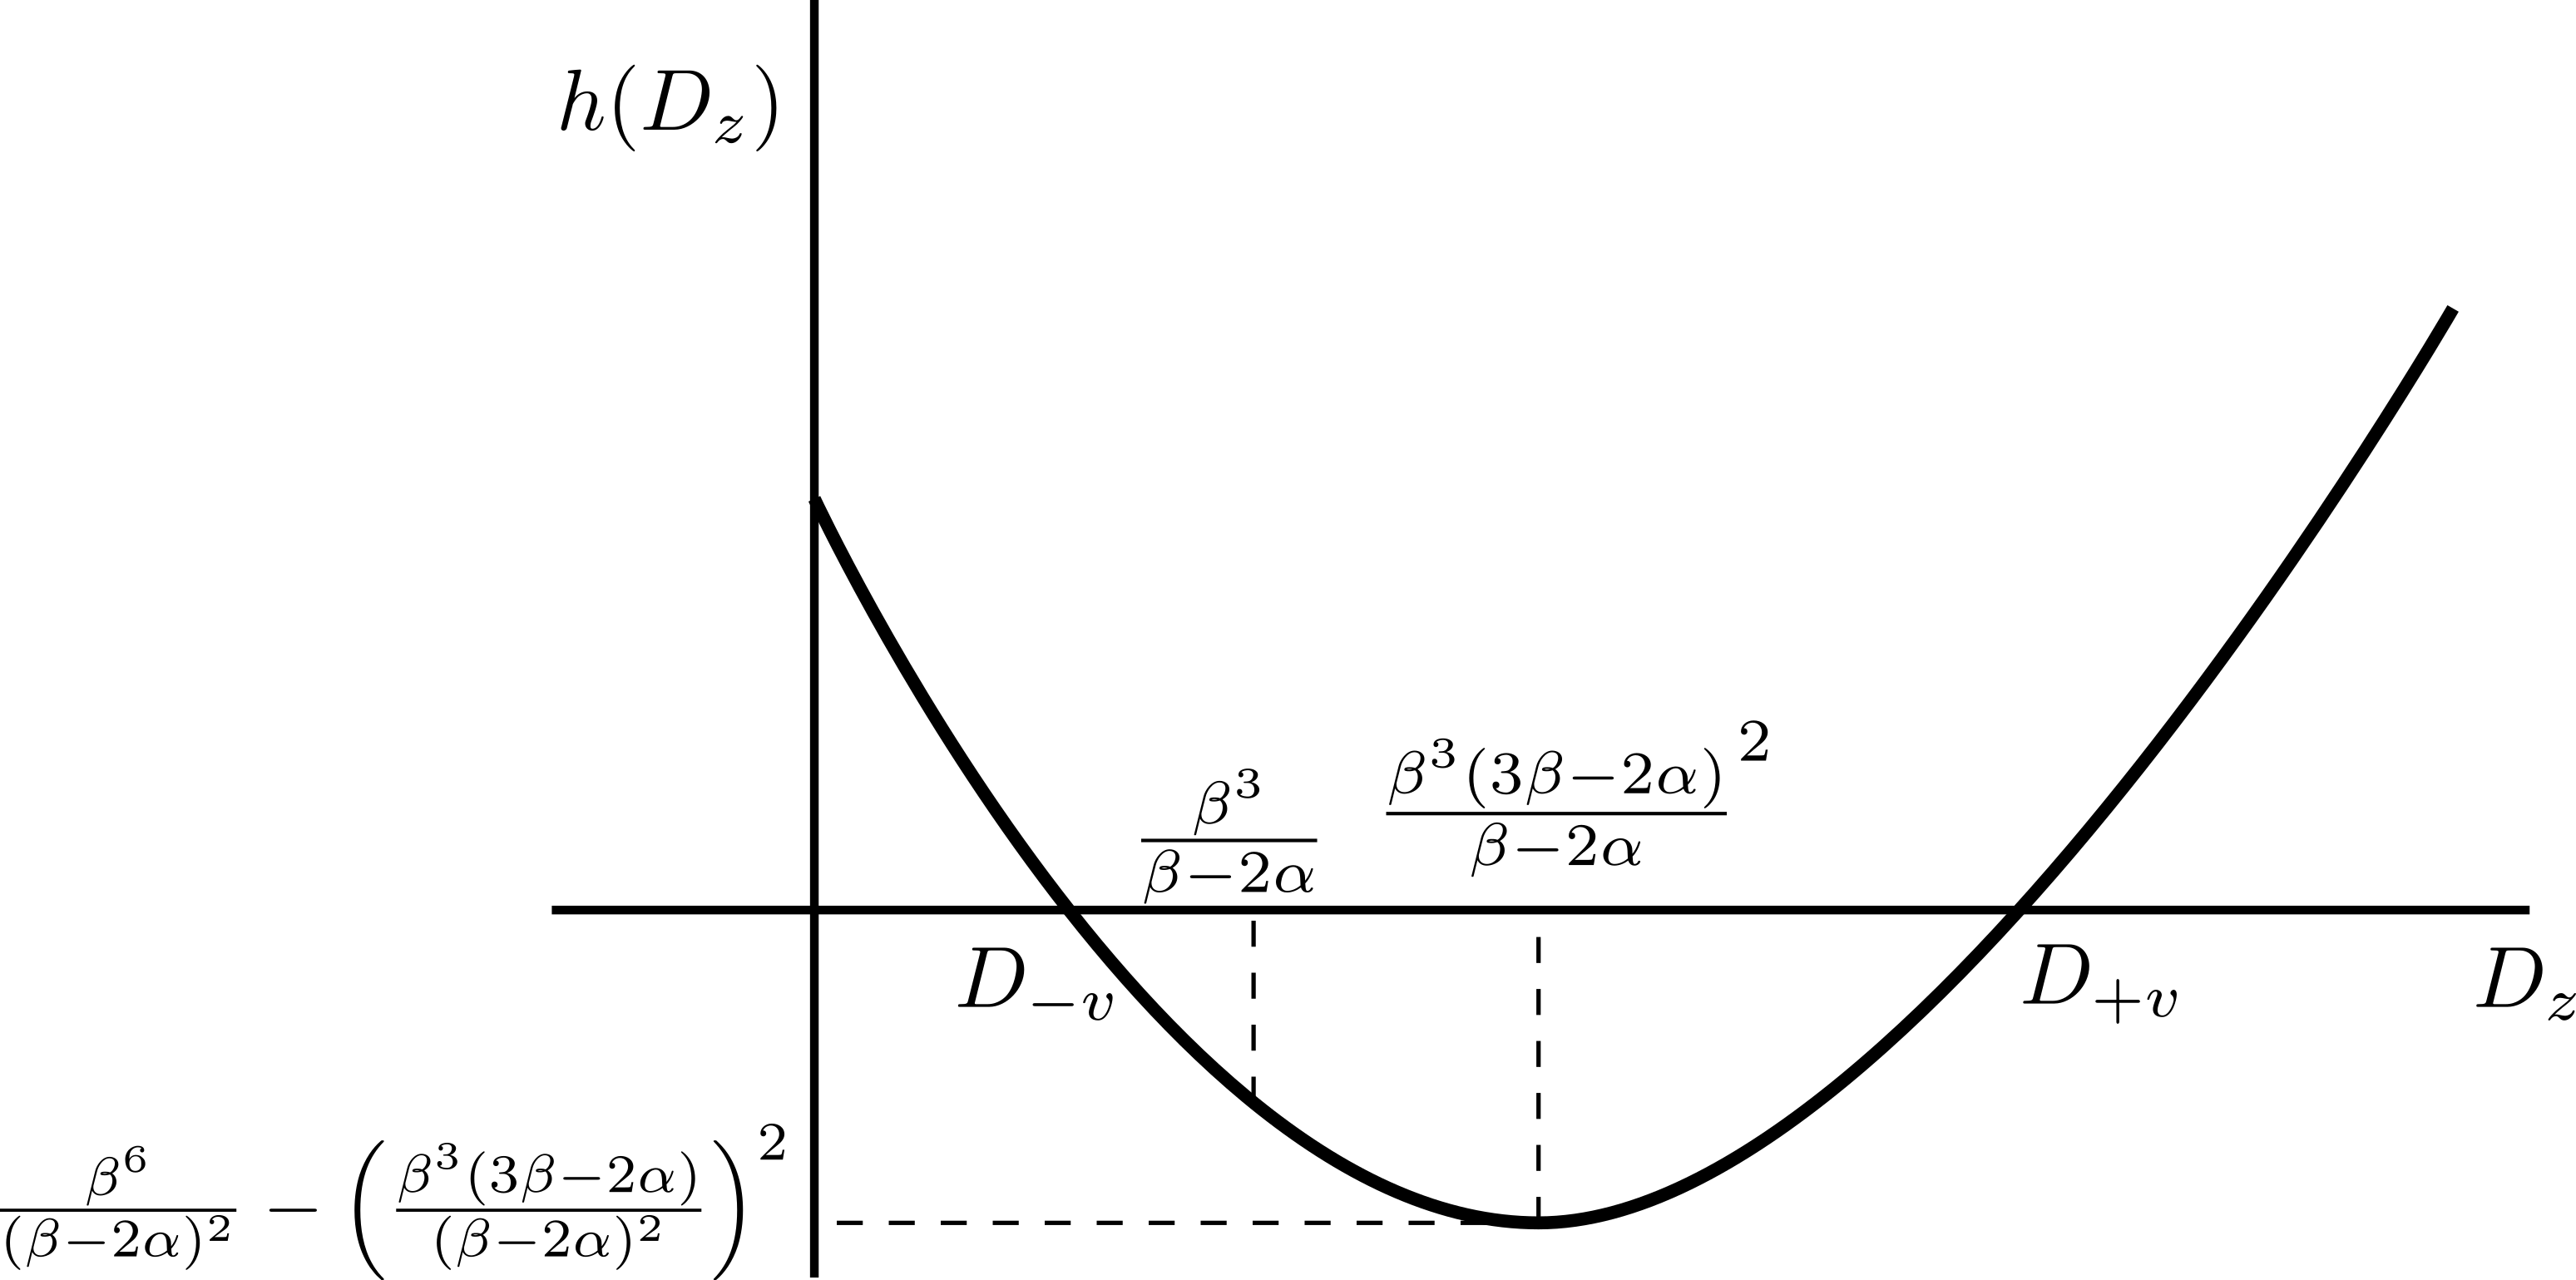
\includegraphics[width=0.8\textwidth]{../Pictures/Schnakeberg_diffusion_curve.png}}
\subfigure[\label{Stable_patterning_region}]{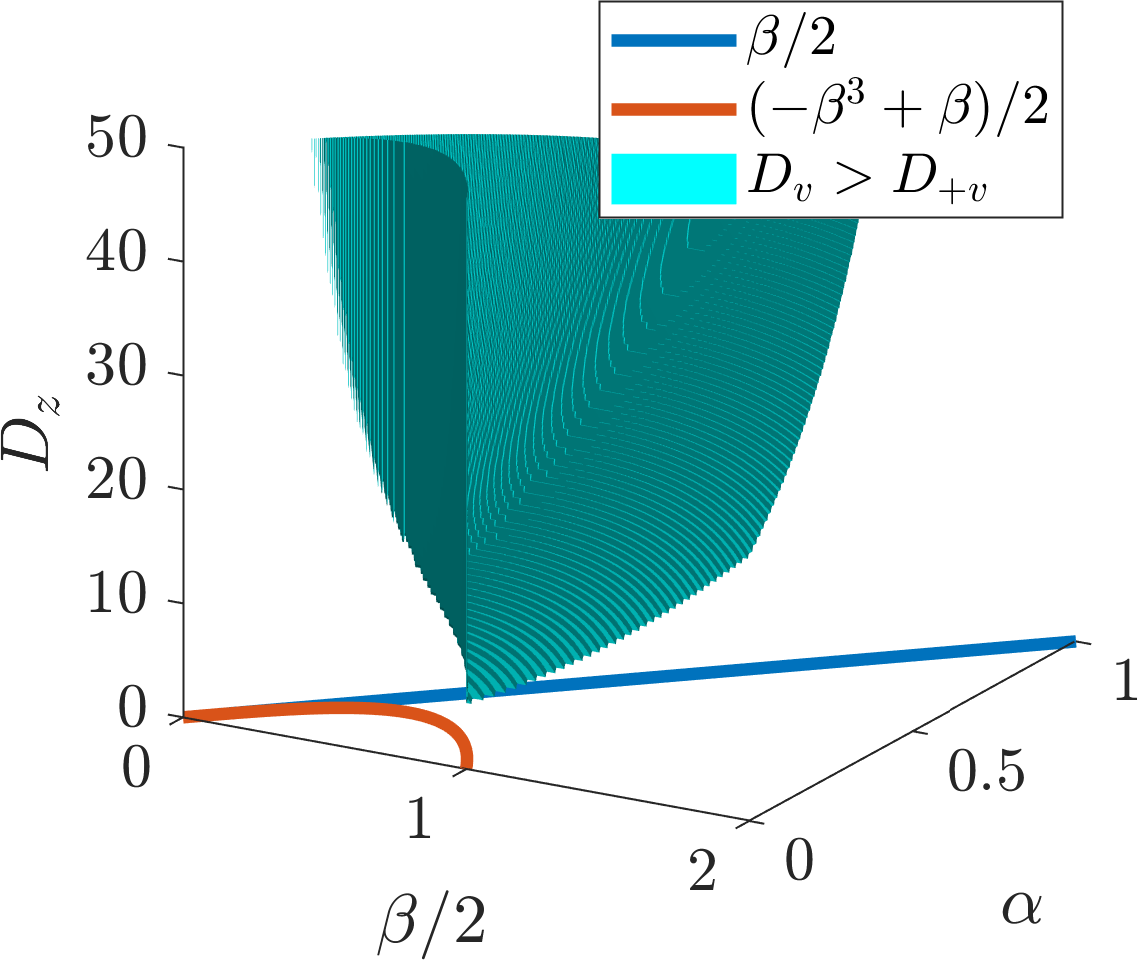
\includegraphics[width=\ttp]{../Pictures/Stable_patterning_region.png}}
\caption{(a) $(\beta,\alpha)$ parameter region, which provides stable homogeneous steady states. (b) Schematic diagram of $h(D_v)$. (c) $(\beta,\alpha,D_v)$ parameter region, which provides diffusion driven unstable homogeneous steady states. \label{DDI_figs}}
\end{figure}
\begin{figure}[!!!h!!!tbp]
\centering
\includegraphics[width=\tp]{../Pictures/Schnak_PDE.png}
\caption{Simulation of \eqns{Schnaku}{Schnakv} with parameters $(\alpha,\beta,D_v,L)=(0.1,0.9,10,5)$. The left image shows the evolving concentration of $u$ over space and time, whilst the right image shows the final heterogeneous solution. \label{Schnak_pde}}
\end{figure}

\subsection{A comment on domain size and spatial dimensions}
From the previous section we can conclude that as the one-dimensional domain gets larger ($L$ increases) higher values of the integer $n$ are valid in \eqn{TT4}. Thus, we would expect that more peaks would appear as the domain gets larger. This is actually observed in nature (see \figs{Goat}{Cow}). However, animal coats are not one-dimensional, thus, we need to consider how our intuition generalises in higher dimensions.  

Consider a Turing system on a two dimensional rectangle with $(x,y)\in [0,L_1]\times [0,L_2]$, zero flux boundary conditions and the Laplacian involving both second spatial derivatives,
\bb
\nabla^2=\DD{}{x}+\DD{}{y}.
\ee
Our perturbation is then of the form
\bb
\l\begin{array}{c} u\\
u
\end {array} \r=\l\begin{array}{c} u_s\\
v_s
\end {array} \r+
\l\begin{array}{c} \epsilon_{u1}\\
\epsilon_{v1}
\end {array} \r\cos(k_xx)\cos(k_yy).
\ee
Following the same procedure as above we find that the allowed values of $k^2$ are now
\bb
k^2=k_x^2+k_y^2 = \frac{m^2 \pi^2}{L_1^2} + \frac{n^2 \pi^2}{L_2^2},
\ee
for some integers $m$ and $n$, excluding the case where they are both zero.

Now, suppose the domain is long and thin, \ie $L_2 \ll L_1$ and $L_1$ is sufficiently large. Then, since we require $k_-<k<k_+$, the only means by which we can have a Turing instability is if $n=0$. Thus, the linear analysis predicts that the patterns are going to be simply spatial oscillations in one dimension. In other words, the pattern will be striped.

For a sufficiently large rectangular domain, where  $L_1 \approx L_2$, we can then satisfy the wave mode criteria with both $n$ and $m>0$. Thus, the linear analysis predicts spatial oscillations in both $x$ and $y$ directions. In other words, the pattern will tend to have a spotted structure \see{Big_and_small_domain}
\begin{figure}[!!!h!!!tbp]
\centering
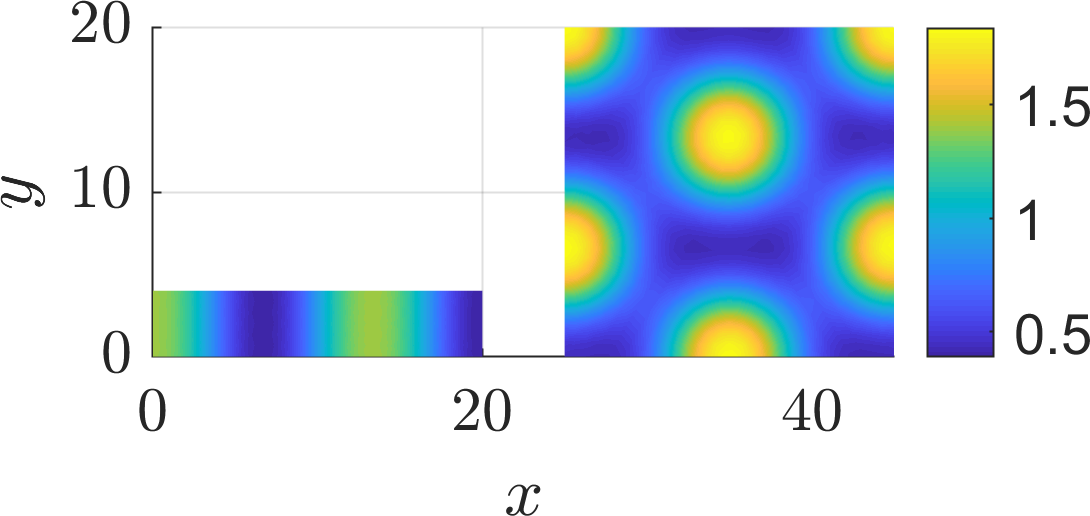
\includegraphics[width=0.8\textwidth]{../Pictures/Big_and_small_domain.png}
\caption{Simulation of \eqns{Schnaku}{Schnakv} with parameters $(\alpha,\beta,D_v)=(0.1,0.9,10)$ on two different two-dimensional domain sizes. \label{Big_and_small_domain}}
\end{figure}

Putting these insights together we see that as the patterning domain gets smaller the patterning type must transition in the following order: spots transform into stripes, which can transform into spatial heterogeneity \see{Tapered_domain}.
 \begin{figure}[!!!h!!!tbp]
\centering
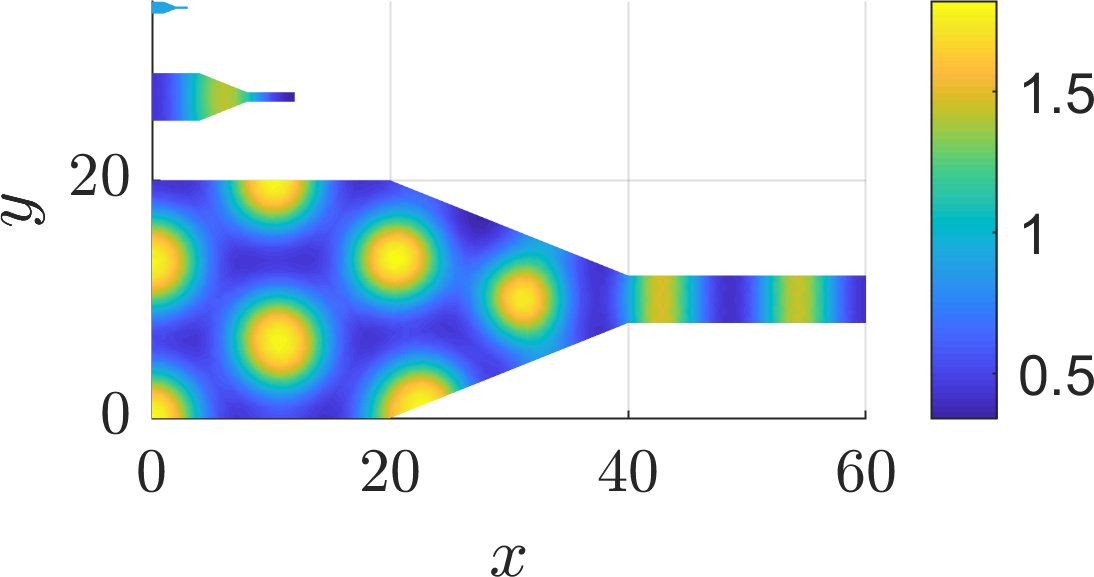
\includegraphics[width=0.8\textwidth]{../Pictures/Tapered_domain.png}
\caption{Simulation of \eqns{Schnaku}{Schnakv} with parameters $(\alpha,\beta,D_v)=(0.1,0.9,10)$ on three sizes of tapered domain \label{Tapered_domain}}
\end{figure}

 Thus, if Turing patterns are behind animal pigmentation patterns we should be able to see animal with spotty bodies and striped tails, but we would not expect to find an animal with a striped body and a spotted tail. Common observations are consistent with such a prediction \see{Genet} but one should not expect universal laws in the realms of biology, as one does in physics \see{Lemur}.
\begin{figure}[!!!h!!!tbp]
\centering
\subfigure[\label{Goat}]{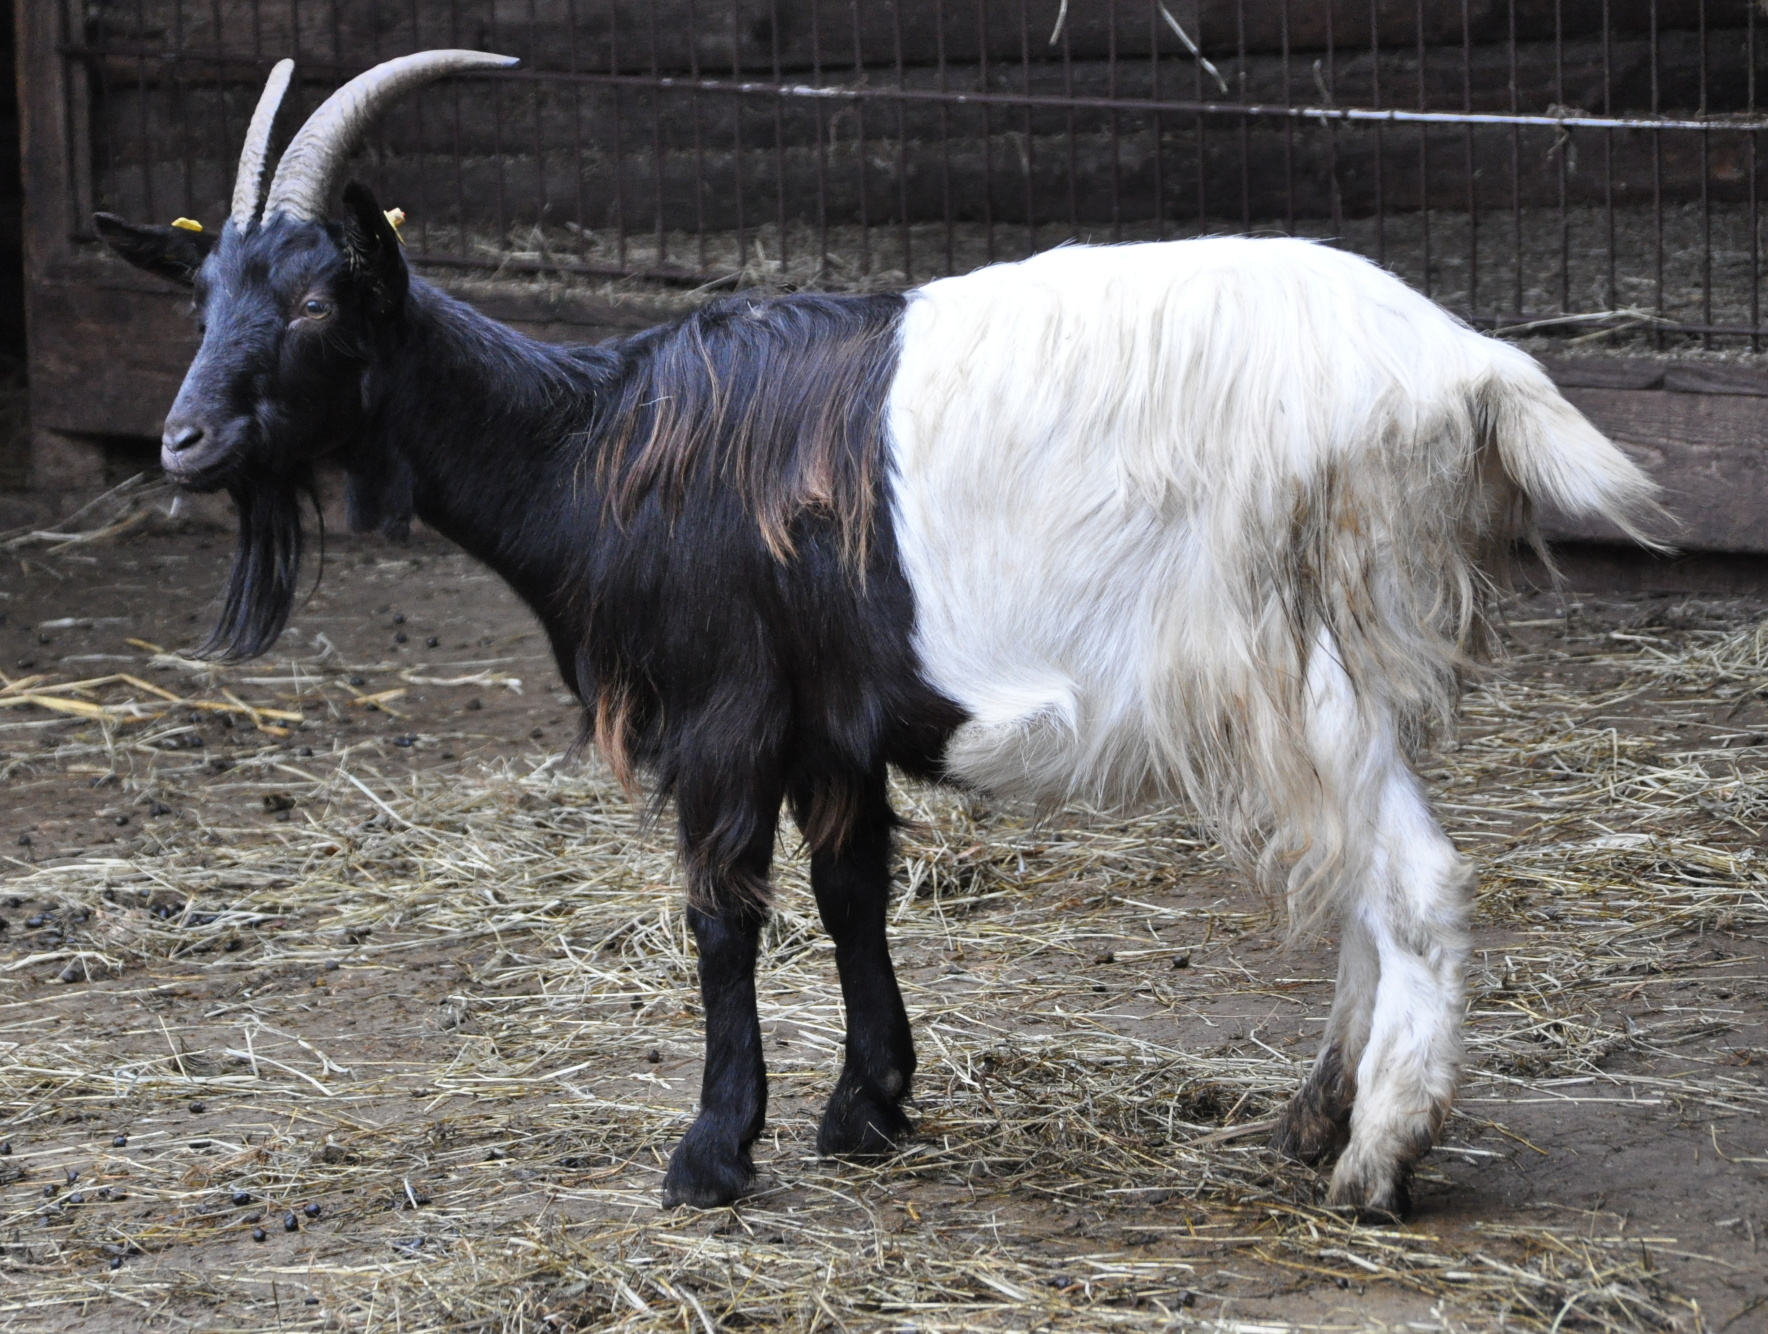
\includegraphics[height=\tttp]{../Pictures/Valais_goat.jpg}}
\subfigure[\label{Cow}]{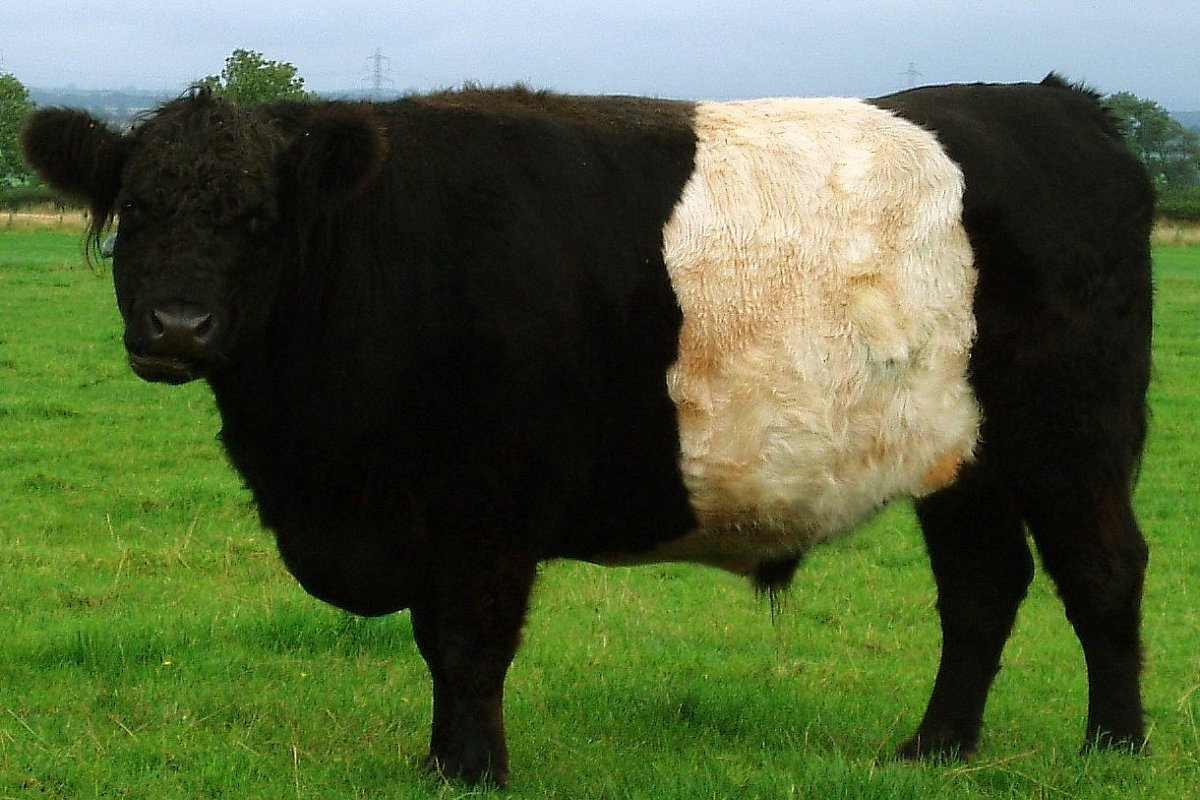
\includegraphics[height=\tttp]{../Pictures/Belted_Galloway.jpg}}
\subfigure[\label{Genet}]{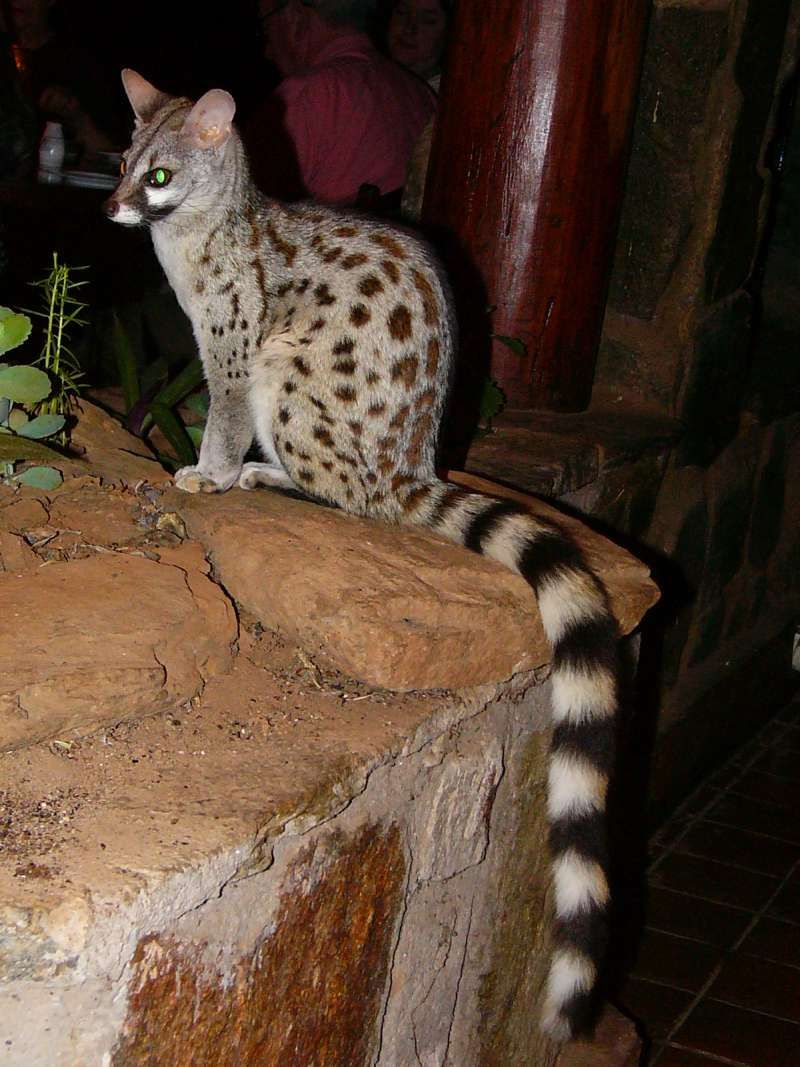
\includegraphics[height=\tttp]{../Pictures/Genet.jpg}}
\subfigure[\label{Lemur}]{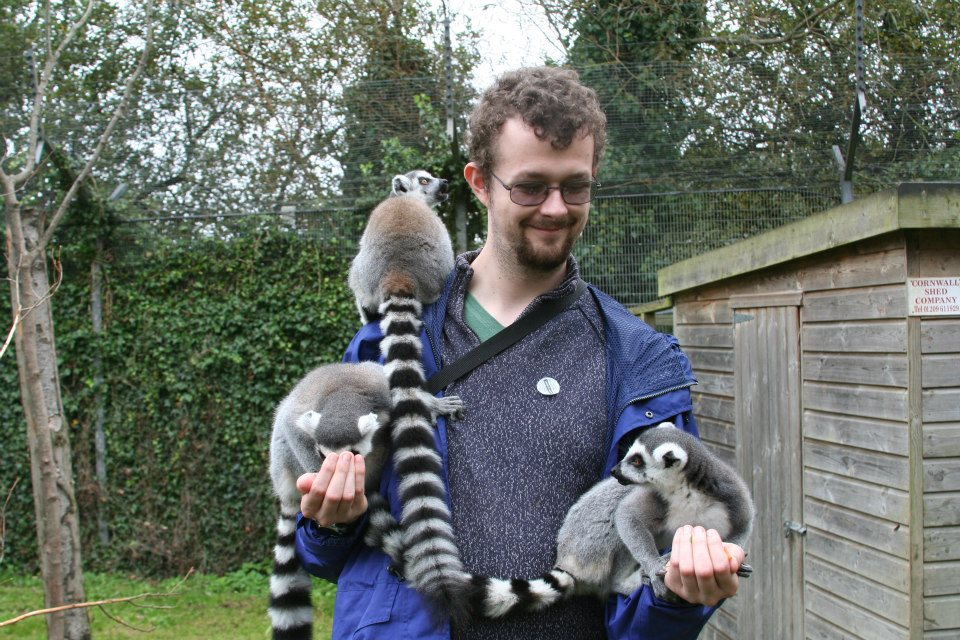
\includegraphics[height=\tttp]{../Pictures/Lemurs.jpg}}
\caption{(a) Valais goats have one stripe transition whereas (b) Belted Galloways have two pigment transitions.(c) The genet cat has a spotted body and striped tail. (d) Lemurs have no pattern on the body and a striped tail. \label{Real_patterns}}
\end{figure}




\section{Do they exist?}
As we have seen, diffusion driven instabilities can theoretically drive pattern formation. Amazingly, there are lots of chemical systems where this is exactly the case \see{Chemical patterns}. Unfortunately, there is yet no conclusive evidence that it can drive pattern formation in biological systems. There are many suggestive pieces of work and many experimental labs are working on isolating the morphogens, but they are still only theoretical in biology. 

Other groups have foregone looking for biological examples and are instead focused on creating there own biological systems that will generate the required conditions in a field called ``synthetic biology''. They are generating a toolbox of biological components that can act like mathematical operators and, thus, they are essentially converting biological problems in computational problems. 
\begin{figure}[!!!h!!!tbp]
\centering
\subfigure[\label{A chemically formed Turing pattern}\href{https://science.sciencemag.org/content/324/5928/772/tab-figures-data}{A chemically formed Turing pattern.}]{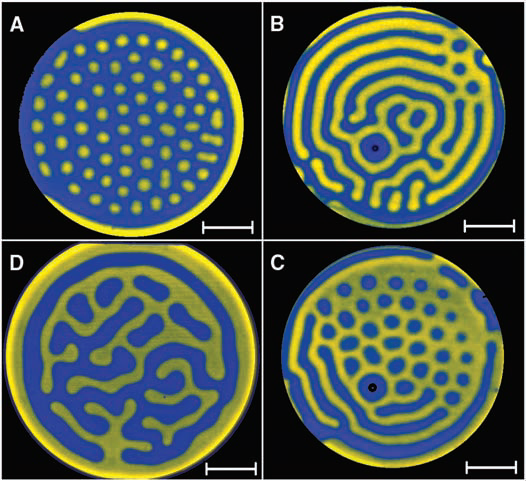
\includegraphics[width=\ttp]{../Pictures/Chemical_turing_patterns.png}}\\
\subfigure[\href{https://www.ncbi.nlm.nih.gov/pmc/articles/PMC4486416/}{Mouse limb development may be governed by a Turing-like patterning process.}\label{Biological_turing_patterns}]{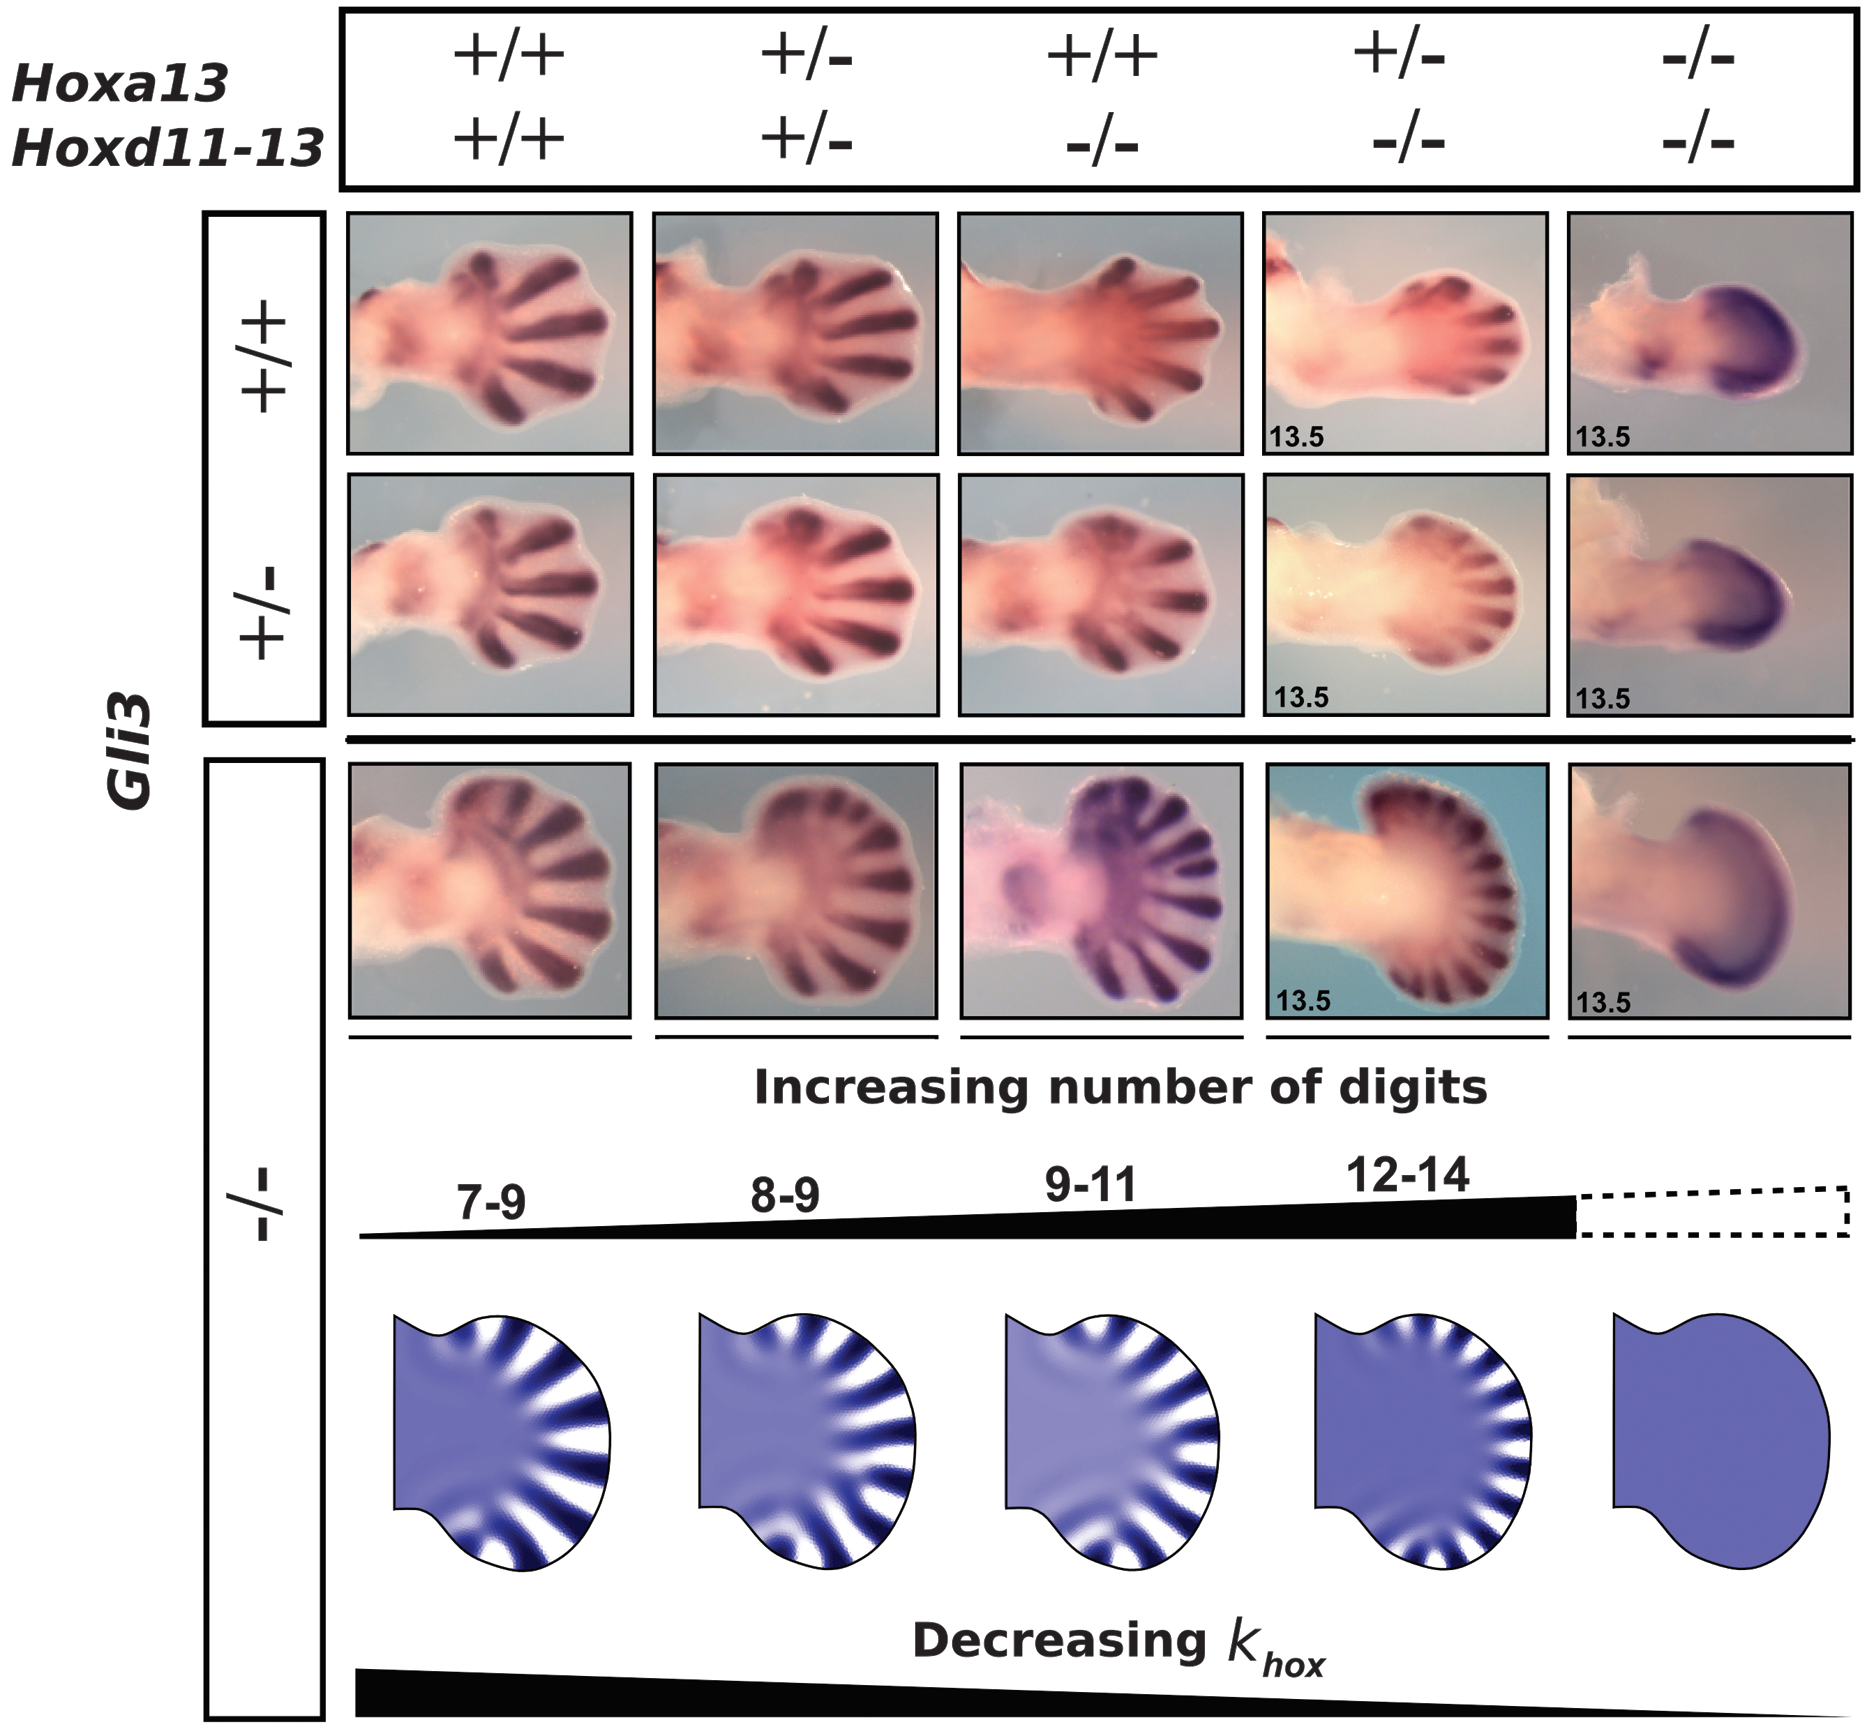
\includegraphics[width=0.8\textwidth]{../Pictures/Biological_turing_patterns.png}}
\caption{Examples of pattern formation in chemistry and biology. Note each subcaption is a link to its source.\label{Chemical patterns}}
\end{figure}

\begin{center}
\textbf{We live in exciting times.}
\end{center}